\documentclass[twoside,a4]{report}
\def\atitle{Development of a Rheometer Controller Using a Raspberry Pi}
\def\shorttitle{Development of a Rheometer Controller}
\def\theauthor{Christopher Boyle}
\def\thewords{10326} % last proper build on Wed 26 April 2017 at 07:46:09
\def\br{\newline \newline \noindent}
\def\hi{\huge{!!!}}
\def\nohi{!!!! \normalsize}
\def\cbh{\large\bfseries !!! ??? !!! \normalsize\normalfont}
%\def\verbatim@font{\linespread{1}\normalfont\ttfamily}
% Imports
\usepackage{fancyvrb}
\usepackage{graphicx}
\usepackage[a4paper]{geometry}
\usepackage{fancyhdr}
\usepackage[english]{babel}
\usepackage{etoolbox}
\usepackage{url}
\usepackage[hidelinks]{hyperref}
\usepackage{subcaption}
\usepackage{nomencl}
\usepackage{calc}
\usepackage{autonum}

% Unused packages
%\usepackage{placeins}
%\usepackage{fancyref}
%\usepackage[comma,authoryear]{natbib}
%\usepackage{lipsum}

% Preamble
\makenomenclature
\renewcommand*{\ttdefault}{qcr}
\renewcommand{\nomlabel}[1]{\hfil #1\hfil}
\nomenclature[a  a]{Symbol}{Description\hfill Units}
\geometry{top=2cm, bottom=2.5cm, left=3cm, right=2.5cm}  % Sets the mnargins
\renewcommand\UrlFont{\rmfamily\itshape}  % sets URL font to normal font (rather than code font)
\setlength{\fboxsep}{2pt}  % separator length around figure boxes
\setlength{\fboxrule}{1pt}  % rule width around figures
\setlength{\parindent}{0pt}
\def\thewords{11866}
\def\achapter{\shorttitle}  % set the command "achapter" to  the name of the current section

\def\nc#1{
	\addtocounter{chapter}{1} 
	\def\achapter{\arabic{chapter} #1}
	\chapter*{\arabic{chapter} #1} 
	\addcontentsline{toc}{chapter}{\achapter} 
}
\def\jc#1{
	\def\achapter{#1}
	\chapter*{\achapter} 
	\addcontentsline{toc}{chapter}{\achapter} 
}

% Header/footer preamble
\fancyhf{}  % clear the current header footer
\fancypagestyle{plain}{  % add settings for plain page style
	\renewcommand{\headrulewidth}{0.4pt}  % weight of the header rule (set to 0 for no line)
	\renewcommand{\footrulewidth}{0.4pt}  % height of the footer rule (set to 0 for no line)
%	\fancyhead[L]{\atitle}  % Header left is title
	\fancyhead[LE]{\achapter}  % Header left (even) is name of chapter
	\fancyhead[RO]{\shorttitle}  % Header right (odd) is report title
	\fancyhead[RE]{\theauthor}  % Header right (even) is author name
	\fancyhead[LO]{University of Strathclyde Chemical Engineering} % Header left (odd) is uni callout
	\fancyfoot[LO]{\today}  % Footer left (odd) is date
	\fancyfoot[RO,LE]{\thepage}  % Footer right (left on even) is page number
}
\pagestyle{plain}

\begin{document}
	%=====------++++++=====------++++++=====------++++++=====------++++++=====------++++++=====------++++++=====------++++++=====------++++++=====------++++++=====------++++++=====------++++++=====------++++++
	%=====------++++++=====------++++++=====------++++++=====------++++++=====------++++++=====------++++++=====------++++++=====------++++++=====------++++++=====------++++++=====------++++++=====------++++++
	%=====------++++++=====------++++++=====------++++++=====------++++++=====------++++++=====------++++++=====------++++++=====------++++++=====------++++++=====------++++++=====------++++++=====------++++++
	%=====------++++++=====------++++++=====------++++++=====------++++++=====------++++++=====------++++++=====------++++++=====------++++++=====------++++++=====------++++++=====------++++++=====------++++++
	%=====------++++++=====------++++++=====------++++++=====------++++++=====------++++++=====------++++++=====------++++++=====------++++++=====------++++++=====------++++++=====------++++++=====------++++++
	%=====------++++++=====------++++++=====------++++++=====------++++++=====------++++++=====------++++++=====------++++++=====------++++++=====------++++++=====------++++++=====------++++++=====------++++++
	%=====------++++++=====------++++++=====------++++++=====------++++++=====------++++++=====------++++++=====------++++++=====------++++++=====------++++++=====------++++++=====------++++++=====------++++++
	%=====------++++++=====------++++++=====------++++++=====------++++++=====------++++++=====------++++++=====------++++++=====------++++++=====------++++++=====------++++++=====------++++++=====------++++++
	\begin{titlepage}
		\makebox[\textwidth][c]{
\includegraphics[scale=1]{images/titleheader.png}}
		\centering
		\vskip3cm
		{
			\bfseries\Large
			Department of Chemical \& Process Engineering\\
			\vskip1cm
			MEng in Chemical \& Process Engineering\\
			18530
			\vskip3cm
			\LARGE\atitle
		}
		\vskip3cm
		{\small Word Count: \thewords}
		\vskip1cm
		\begin{flushleft}
			This project is submitted in partial fulfilment of the regulations governing the award of \\
			Degree of MEng in Chemical Engineering at the University of Strathclyde
			\vskip2cm
			Author: Christopher Boyle \hfill Date: \today \newline
			\vskip1cm
			Organisation: University of Strathclyde, Department of Chemical \& Process Engineering \newline
			%In-house Supervisor: Dr. Leo Lue \newline% \newline
			Academic Supervisor: Dr. Leo Lue
		\end{flushleft}
	\end{titlepage}

	%=====------++++++=====------++++++=====------++++++=====------++++++=====------++++++=====------++++++=====------++++++=====------++++++=====------++++++=====------++++++=====------++++++=====------++++++
	%=====------++++++=====------++++++=====------++++++=====------++++++=====------++++++=====------++++++=====------++++++=====------++++++=====------++++++=====------++++++=====------++++++=====------++++++
	%=====------++++++=====------++++++=====------++++++=====------++++++=====------++++++=====------++++++=====------++++++=====------++++++=====------++++++=====------++++++=====------++++++=====------++++++
	%=====------++++++=====------++++++=====------++++++=====------++++++=====------++++++=====------++++++=====------++++++=====------++++++=====------++++++=====------++++++=====------++++++=====------++++++
	%=====------++++++=====------++++++=====------++++++=====------++++++=====------++++++=====------++++++=====------++++++=====------++++++=====------++++++=====------++++++=====------++++++=====------++++++
	%=====------++++++=====------++++++=====------++++++=====------++++++=====------++++++=====------++++++=====------++++++=====------++++++=====------++++++=====------++++++=====------++++++=====------++++++
	%=====------++++++=====------++++++=====------++++++=====------++++++=====------++++++=====------++++++=====------++++++=====------++++++=====------++++++=====------++++++=====------++++++=====------++++++
	%=====------++++++=====------++++++=====------++++++=====------++++++=====------++++++=====------++++++=====------++++++=====------++++++=====------++++++=====------++++++=====------++++++=====------++++++
	%Post title settings
	\pagenumbering{roman}
	\setcounter{page}{0}
	\begin{center}\newpage \end{center}
	
	%=====------++++++=====------++++++=====------++++++=====------++++++=====------++++++=====------++++++=====------++++++=====------++++++=====------++++++=====------++++++=====------++++++=====------++++++
	%=====------++++++=====------++++++=====------++++++=====------++++++=====------++++++=====------++++++=====------++++++=====------++++++=====------++++++=====------++++++=====------++++++=====------++++++
	%=====------++++++=====------++++++=====------++++++=====------++++++=====------++++++=====------++++++=====------++++++=====------++++++=====------++++++=====------++++++=====------++++++=====------++++++
	%=====------++++++=====------++++++=====------++++++=====------++++++=====------++++++=====------++++++=====------++++++=====------++++++=====------++++++=====------++++++=====------++++++=====------++++++
	%=====------++++++=====------++++++=====------++++++=====------++++++=====------++++++=====------++++++=====------++++++=====------++++++=====------++++++=====------++++++=====------++++++=====------++++++
	%=====------++++++=====------++++++=====------++++++=====------++++++=====------++++++=====------++++++=====------++++++=====------++++++=====------++++++=====------++++++=====------++++++=====------++++++
	%=====------++++++=====------++++++=====------++++++=====------++++++=====------++++++=====------++++++=====------++++++=====------++++++=====------++++++=====------++++++=====------++++++=====------++++++
	%=====------++++++=====------++++++=====------++++++=====------++++++=====------++++++=====------++++++=====------++++++=====------++++++=====------++++++=====------++++++=====------++++++=====------++++++
	% Summary
	\jc{Summary}
	
	%Brief, factual, generally following the same order of presentation as the report. Do not include figures, tables, or references.
	The aim of this project was to design, build, and test a rheometer. The rheometer is to be used to examine closely the time varying properties of a jammed system. Jamming is where a shearing fluid has a discontinuous jump up in apparent viscosity such that it no longer acts like a fluid - it acts like a solid. The rheometer was designed around a Couette cell - two concentric cylinders with a liquid in the gap between the two. One cylinder is rotated to shear the fluid (the other fixed), the rate of rotation and the torque are used to calculate the viscosity. The rheometer was managed and controlled by a Raspberry Pi computer, which uses information from sensors to calculate the viscosity. The rheometer was to meet certain criteria. The finished rheometer should:
	\begin{itemize}
		\item be able to calculate the viscosity of a fluid as it varies with time.
		\item be operationally modular (easy to alter the exact parameters with which it runs).
		\item be low-cost (under \pounds 100).
	\end{itemize}
	The main hardware was a Taylor-Couette shear cell. Electronic circuits were designed to automatically and precisely control the motor (used to shear the fluid). Also developed were several sensors used to read the data necessary to calculate the viscosity. Software was written to allow the Raspberry Pi to manage and communicate with the hardware. 
	\br
	The rheometer was tested by using it to measure the viscosity of reference Newtonian fluids (aqueous solutions of Glycerol) to evaluate the its ability to accurately gauge a fluid's viscosity.  The use of colloidal suspensions to evaluate the validity of the rheometer will be future work.
	
	
	\newpage \begin{center} \large \space \normalsize \end{center}
	
	%=====------++++++=====------++++++=====------++++++=====------++++++=====------++++++=====------++++++=====------++++++=====------++++++=====------++++++=====------++++++=====------++++++=====------++++++
	%=====------++++++=====------++++++=====------++++++=====------++++++=====------++++++=====------++++++=====------++++++=====------++++++=====------++++++=====------++++++=====------++++++=====------++++++
	%=====------++++++=====------++++++=====------++++++=====------++++++=====------++++++=====------++++++=====------++++++=====------++++++=====------++++++=====------++++++=====------++++++=====------++++++
	%=====------++++++=====------++++++=====------++++++=====------++++++=====------++++++=====------++++++=====------++++++=====------++++++=====------++++++=====------++++++=====------++++++=====------++++++
	%=====------++++++=====------++++++=====------++++++=====------++++++=====------++++++=====------++++++=====------++++++=====------++++++=====------++++++=====------++++++=====------++++++=====------++++++
	%=====------++++++=====------++++++=====------++++++=====------++++++=====------++++++=====------++++++=====------++++++=====------++++++=====------++++++=====------++++++=====------++++++=====------++++++
	%=====------++++++=====------++++++=====------++++++=====------++++++=====------++++++=====------++++++=====------++++++=====------++++++=====------++++++=====------++++++=====------++++++=====------++++++
	%=====------++++++=====------++++++=====------++++++=====------++++++=====------++++++=====------++++++=====------++++++=====------++++++=====------++++++=====------++++++=====------++++++=====------++++++
	% Contents Page
	\newpage
	\def\achapter{Contents}
	\tableofcontents
	\jc{Acknowledgements} 
	%IT is a matter of honesty and courtesy that acknowledgement is made to those who helped you in your work.
	First, I'd like to thank Dr. Leo Lue for his help and inspiration throughout this project.
	\br
	I'd like to thank Aditi Mukhopadhyay for her help and encouragement over the last few months! Also for her essential aid in the lab using the DHR-2.
	\br
	Special thanks to Jim Murphy, who made the Couette cylinders himself, and I'd also like to thank Christopher Jones help with the lab equipment.
	\br
	Finally, I'd like to thank the communities of the internet for telling me where I was going wrong. I would still be trying to spin a motor if not for the great help from the StackExchange forum. 
	
	\newpage
	\pagenumbering{arabic}
	\setcounter{page}{1}
	
	%=====------++++++=====------++++++=====------++++++=====------++++++=====------++++++=====------++++++=====------++++++=====------++++++=====------++++++=====------++++++=====------++++++=====------++++++
	%=====------++++++=====------++++++=====------++++++=====------++++++=====------++++++=====------++++++=====------++++++=====------++++++=====------++++++=====------++++++=====------++++++=====------++++++
	%=====------++++++=====------++++++=====------++++++=====------++++++=====------++++++=====------++++++=====------++++++=====------++++++=====------++++++=====------++++++=====------++++++=====------++++++
	%=====------++++++=====------++++++=====------++++++=====------++++++=====------++++++=====------++++++=====------++++++=====------++++++=====------++++++=====------++++++=====------++++++=====------++++++
	%=====------++++++=====------++++++=====------++++++=====------++++++=====------++++++=====------++++++=====------++++++=====------++++++=====------++++++=====------++++++=====------++++++=====------++++++
	%=====------++++++=====------++++++=====------++++++=====------++++++=====------++++++=====------++++++=====------++++++=====------++++++=====------++++++=====------++++++=====------++++++=====------++++++
	%=====------++++++=====------++++++=====------++++++=====------++++++=====------++++++=====------++++++=====------++++++=====------++++++=====------++++++=====------++++++=====------++++++=====------++++++
	%=====------++++++=====------++++++=====------++++++=====------++++++=====------++++++=====------++++++=====------++++++=====------++++++=====------++++++=====------++++++=====------++++++=====------++++++
	% Introduction
	\nc{Introduction}
	
	% BACKGROUND AND MOTIVATION
	This project aimed to design, build, and test a control system for a bespoke rheometer which will focus on recording time varying properties of colloidal suspensions in order to better understand jamming. Jamming is a form of discontinuous shear thickening where a fluid experiencing shear appears to become solid. This causes problems in pharmaceuticals, food processing; industries where powders and suspensions are common. Jamming mainly causes transportation and mixing problems - situations where the fluid is sheared. With better understanding of how jamming comes about, a better understanding of the rules governing it, more efficient and more effective techniques can be developed to better manage a jammed system (reduce the likelihood of jams, improve efficiency of jam disruption methods).
	\br
	% OBJECTIVES & DESIGN CRITERIA
	The rheometer will be used to examine jamming events in colloidal suspensions in order to obtain more information - focussing in on time varying aspects of the jam - how often does the suspension jam? How is this jamming frequency related to the shear stress or strain rate experienced by the fluid? The rheometer mainly consists of a Taylor-Couette shear cell - two concentric cylinders between which is the fluid to be tested. The final design should:
	\begin{itemize}
		\item be able to calculate the viscosity of a fluid as it varies with time.
		\item be operationally modular (easy to alter the exact parameters with which it runs).
		\item be low-cost (under \pounds 100).
	\end{itemize}
	Being able to measure the viscosity of a fluid with respect to time is an important consideration. This is the main criteria for the project. The modularity of the script would make the device useful beyond just a jamming rheometer (a rheometer able to automatically reset and perform another experiment under different conditions, for example). Finally, the cost constraint makes the rheometer attractive as an alternative to other (pre-existing) devices that could be used in the same situation: ``from about \$40,000 for an 'entry-level' rheometer to `upwards of \$200,000' for a full-featured and fully configurable research-level system" \cite{refrheomprice}.
	\br
	The hardware was controlled by a Raspberry Pi computer. This computer (originally developed as an educational item, to better computing skills in students) is around the size of a credit card, uses micro-USB for power, and can directly communicate with hardware over its General Purpose Input-Output ports (GPIO).
	The hardware connected to the Raspberry Pi was relatively simply: a programmable motor driver circuit, and two sensors (one for rotational speed, and another for motor current supply).\br
	The rheometer itself was a Taylor-Couette shear cell rheometer composed of two cylinders; the outer one hollow and contained the fluid; the inner one solid. The inner cylinder is rotated to shear the fluid. Sensors were used to detect the torque and speed involved in rotating the cylinder, information which is used to calculate the viscosity. The rheometer's ability to measure viscosity by using it to test the viscosity of several newtonian fluids of known viscosity (as tested in a laboratory rheometer).
	\br 
	This report summarises the final design at the end of the 12 week long project. Chapter 2 gives background information on the concepts involved (the Raspberry Pi, non-Newtonian fluids and jamming). Chapter 3 is a detailed description of the methods involved in the project; how the hardware was put together, what software was written, and how the calibrations and evaluations were undertaken. Chapter 4 evaluates the final build of the rheometer against the design criteria and discusses where it fell short and how improvements may be made. Chapter 5 consists of concluding remarks about the procedure; a summary of the results that were found, an evaluation of the final device, and a summary of future work. Chapter 6 gives my personal reflection on the project, how I have learned from the process, and what I felt could have been done better.
	%This report summarises the final design at the end of the 12 week long project. Chapter 2 gives background information on the concepts involved (the Raspberry Pi, non-Newtonian fluids and jamming). Chapter 3 gives a background on the University of Strathclyde and the Chemical and Process Engineering Department. Chapter 4 is a detailed description of the methods involved in the project; how the hardware was put together, what software was written, and how the calibrations and evaluations were undertaken. Chapter 5 evaluates the final build of the rheometer against the design criteria and discusses where it fell short and how improvements may be made. Chapter 6 consists of concluding remarks about the procedure; a summary of the results that were found, an evaluation of the final device, and a summary of future work. Chapter 7 gives my personal reflection on the project, how I have learned from the process, and what I felt could have been done better.
	
	%=====------++++++=====------++++++=====------++++++=====------++++++=====------++++++=====------++++++=====------++++++=====------++++++=====------++++++=====------++++++=====------++++++=====------++++++
	%=====------++++++=====------++++++=====------++++++=====------++++++=====------++++++=====------++++++=====------++++++=====------++++++=====------++++++=====------++++++=====------++++++=====------++++++
	%=====------++++++=====------++++++=====------++++++=====------++++++=====------++++++=====------++++++=====------++++++=====------++++++=====------++++++=====------++++++=====------++++++=====------++++++
	%=====------++++++=====------++++++=====------++++++=====------++++++=====------++++++=====------++++++=====------++++++=====------++++++=====------++++++=====------++++++=====------++++++=====------++++++
	%=====------++++++=====------++++++=====------++++++=====------++++++=====------++++++=====------++++++=====------++++++=====------++++++=====------++++++=====------++++++=====------++++++=====------++++++
	%=====------++++++=====------++++++=====------++++++=====------++++++=====------++++++=====------++++++=====------++++++=====------++++++=====------++++++=====------++++++=====------++++++=====------++++++
	%=====------++++++=====------++++++=====------++++++=====------++++++=====------++++++=====------++++++=====------++++++=====------++++++=====------++++++=====------++++++=====------++++++=====------++++++
	%=====------++++++=====------++++++=====------++++++=====------++++++=====------++++++=====------++++++=====------++++++=====------++++++=====------++++++=====------++++++=====------++++++=====------++++++
	% Background
	\nc{Background}	
	\section*{Rheometry}
	The viscosity of a fluid is a measure of how resistant it is to flow. This is an important concept in process engineering: most processes involve fluids, many products have fluid components. The viscosity (\(\mu\)) of a fluid can be calculated from the shear stress (\(\tau\)) imposed on a fluid and the rate at which it deforms (shear rate, \(\dot{\gamma}\)) using Newton's Law of Viscosity (Equation \ref{eqnvisco}) \cite{backfluidmech}.
	\begin{equation}
	\mu = \frac{\tau}{\dot{\gamma}}
	\label{eqnvisco}
	\end{equation}
	There are different classes of fluids depending on how their viscosity behaves with respect to shear rate or to shear stress. Newtonian fluids have a constant viscosity, the shear stress required to shear at a specific rate is directly proportional to the shear rate and the fluid's viscosity is the constant of proportionality. Non-Newtonian fluids have viscosities that are not constant. Some fluids viscosities which vary with the length of time shear is applied. Thixotropic fluids have a viscosity which apparently reduces the longer a stress is applied. Rheopectic fluids have a viscosity which apparently increases the longer a stress is applied. Other non-Newtonian fluids' viscosity is dependent on the magnitude of the stress. Shear-thinning fluids have a viscosity that appears to decrease with increased stress. Shear thickening fluids appear to experience a viscosity increase with an increase in stress \cite{backtypesofnonnewt}. Figures \ref{figshearthin} \& \ref{figshearthick} give examples of how shear rate varies with shear stress for non-Newtonian fluids. 
	\br
	\begin{figure}[!htb]
		\centering
		\begin{subfigure}[t]{0.45\textwidth}
			\centering
			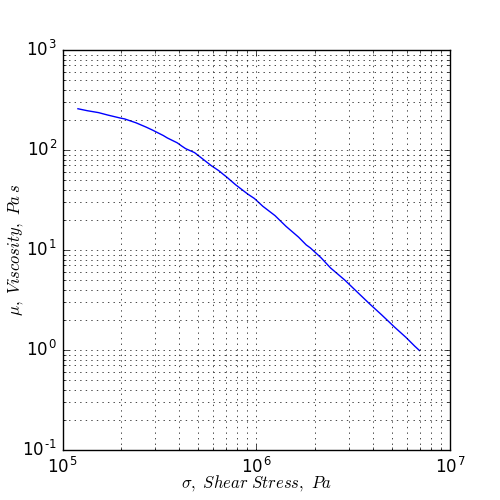
\includegraphics[scale=0.5]{figures/fig_shear_behav_thin.png}
			\caption{Shear Thinning}
			\label{figshearthin}
			\footnotesize 
			Viscosity vs. shear stress for a shear-thinning fluid. Glass spheres 15 $\mu$m in diameter suspended in thermoplastic.
		\end{subfigure}
		\begin{subfigure}[t]{0.45\textwidth}
			\centering
			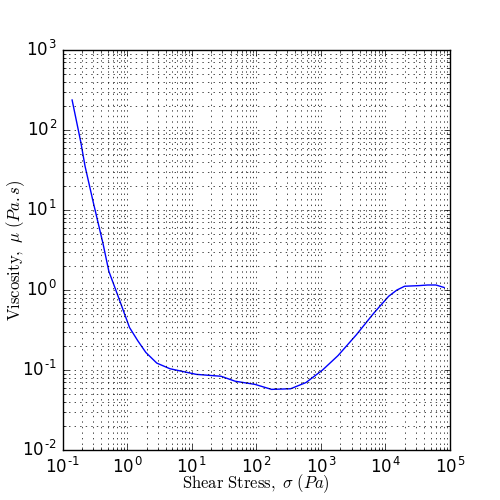
\includegraphics[scale=0.5]{figures/fig_shear_behav_thick.png}
			\caption{Shear Thickening}
			\label{figshearthick}
			\footnotesize 
			Viscosity vs. Shear stress for a shear thickening fluid ($\phi=0.5$, colloidal latex particles dispersed in water). The initial shear thinning region can be seen before the fluid acts Newtonian until the shear stress reaches a critical yield stress and the fluid appears to thicken. At high stress, the fluid once again acts Newtonian.
		\end{subfigure}
		\label{figshearthinthick}
		\caption{Viscosity vs Shear Stress (adapted from \cite{figshearthin, figshearthick})}
	\end{figure}
	
	\noindent
	Viscosity is measured in the lab using a rheometer. There are three general types of rheometers: capillary, cone-and-plate, and rotational. Capillary rheometers consist of a tube of known cross section, through which the test fluid is forced (by pumping, by piston). The viscosity can be found by measuring the flow rate and pressure gradient, and using the Hagen-Poiseulle equation for laminar flow through a pipe \cite{backcaprheom}. Cone-and-plate rheometers consist of a cone rotating in fluid on a stationary plate. The torque required to spin the cone at a speed is measured. The shear stress in the fluid is proportional to the torque output by the motor, and the shear rate is proportional to the rotation rate. 
	\br
	The rotational rheometer is based upon the idea of Couette flow: two infinitely long plates (separated by a known amount) between which is fluid. As one plate moves, the fluid is sheared. In Couette flow, the strain rate calculation is simplified: strain rate is the first derivative of the velocity of the shear. In Couette flow, the velocity varies linearly with across the gap therefore the strain rate is constant. A Couette cell is a practical approximation of the infinitely long plate shear scenario. The cell is constructed from two cylinders: the outer cylinder and the inner cylinder. The cylinders are positioned vertically close together to limit the amount of fluid shearing on the bottom of the inner cylinder. This set up mimics the Couette flow idea and closely replicates the effect, resulting in linear variation of velocity, and a constant strain rate \cite{couetteshearcell}.
	\br
	The Taylor-Couette shear cell built in this project uses a DC motor as a transducer to both read shear stress information from the cell and to provide the shearing force. Calibrations and characteristics of the motor used are used in order to calculate the information required to obtain the viscosity of the fluid in the shear cell.
	\begin{figure}[!htb]
		\centering
		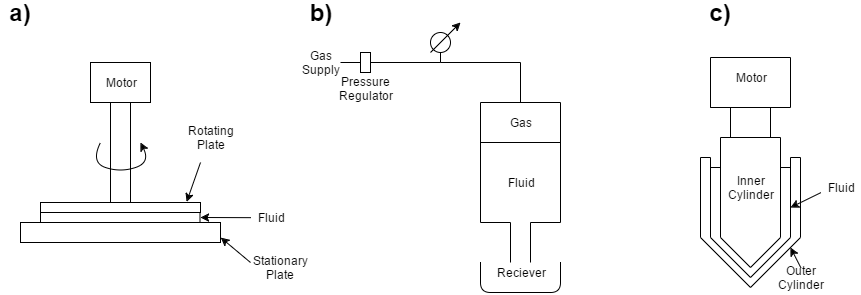
\includegraphics[scale=0.45]{images/capschem.png}
		\caption{Rheometer Schematics}
		\label{figrheomschem}
		\footnotesize 
		\textbf{(a)} Cone-and-plate rheometer schematic (adapted from \cite{tadhrbrochure})\\
		\textbf{(b)} Capillary rheometer schematic (adapted from \cite{figcapschem})\\
		\textbf{(c)} Taylor-Couette shear cell rheometer schematic (adapted from \cite{couetteshearcell})
	\end{figure}
	
	\section*{Colloidal Suspensions and Jamming}
	Fluids consisting of solid particles suspended in a liquid are prone to non-Newtonian behaviour, most commonly shear thinning. Some suspensions exhibit shear thickening behaviour. The concept of hydroclustering has been used to explain this shear thickening behaviour: as the suspension undergoes shear, the particles are forced together forming larger particle groups. This increases the effective viscosity compared to low shear flow where the particles movements are not as restricted \cite{figshearthick}. The order-disorder transition  theory explains the increase in viscosity as being due to an increase in stress causing the particles to become disordered. Initially there is a drop in viscosity, due to the particles in the suspension becoming more ordered. Then, as the stress is increased past a yield stress, the viscosity begins to increase due to a disruption in the order of the particles \cite{backbrownjaegrev}. % other theories?
	\br
	Shear thickening can be split further into continuous shear thickening (CST) and discontinuous shear thickening (DST). In CST the viscosity increases proportionally to shear after a yield stress. However, with DST the viscosity suddenly (almost asymptotically) jumps upwards. DST has been associated with an apparent decrease in volume fraction of suspensions - hence its alternative name of dilatency. This effect also supports the order-disorder-transition theory of shear thickening: you would expect the volume fraction to decrease (void fraction to increase) if the particles are going from a neat, ordered arrangement into extreme disorder \cite{backbrownjaegrev}. 
	\br
	DST is linked to the concept of jamming, which is \textit{``the conversion of a liquid system into a solid by imposed stress"} \cite{backhawjam}. Jamming is found in many different systems: in solids entering a hopper \cite{back2djam}, in pedestrians walking down a corridor \cite{backpedjam}, and in traffic \cite{backcarjam}. This can cause problems in processes: halting flow, damaging mixing equipment \cite{backshearjambertrand}.
	\br 
	An interesting phenomenon that occurs in jamming suspensions is the formation and dissipation of ``cracks" on the surface of the suspension. This can be directly seen in Figure \ref{cforscracks}. The cracks have been associated with a localized change in volume faction of the suspended particles \cite{backhawjam}. Another interesting optical property of jammed suspensions: the surface of a shear suspension has been found to alter texture, evidence of ``dilation" \cite{backbrownjaegrev}: caused by the particles in shear attempting to move around each other but having to take an inefficient route therefore decreasing the volume fraction of the suspension. This draws more fluid into the bulk and then the surface appears rough in texture, as opposed to glossy. 
	
	\begin{figure}[!htb]
		\centering
		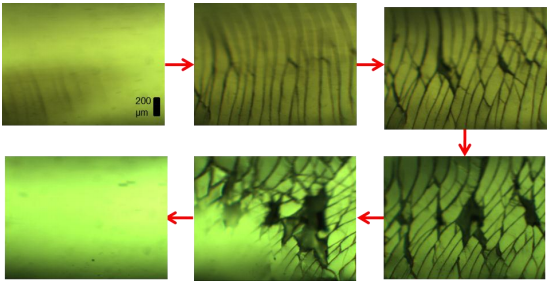
\includegraphics[scale=0.45]{images/cfors_cracks.png}
		\caption{Suspension Surface Cracks (taken from \cite{thescforsyth})}
		\label{cforscracks}
	\end{figure}

	\section*{DC Motor}
	DC motors use the current flowing through coils of wire to create a magnetic field. This field acts against permanent magnets within the motor creating a force pushing on the coils. The coils are mounted in a rotating structure called an armature. This is set up such that as the coil produces a field of one polarity in the direction of the magnet, the coil is pushed away from a magnetic pole and pulled towards its polar opposite. But as it passes this magnet to which it is attracted, the supply is switched within the motor causing the flow of current in the coil to reverse and thus the polarity of the magnetic field produced. The coil is then pushed away from the magnetic pole, and towards its polar opposite. This procedure is undergone by several coils in an optimal pattern within the motor to produce a constant velocity \cite{backdcmotor}.
	\br
	The behaviour of the motor can be predicted using characteristic equations. These equations describe how the motor performs under load at a supply voltage. Figure \ref{figmotcharexample} is an example of a plot of these characteristic equations for a DC motor. At the right hand side, the torque is the stall torque --- a load high enough to halt movement of the motor. At the left hand side, the motor is unloaded and the speed is at a maximum --- the no-load speed. This plot is for a single supply voltage: the stall torque and supply voltage both vary with voltage. 
	\br
	It can be seen that the current draw line does not pass through the origin - there is some `minimum' current. This `minimum' current is the current drawn by the voltage passing through the coils ($I_{coil}$) in the motor - by Ohm's law ($V = I \times R$) this varies with voltage by the resistance of the coils. The 'top' current (or EMF current, $I_{emf}$) on top of the coil current is the current drawn by the magnetic field of the coils acting against the magnetic fields of the permanent magnets within the motor. If nothing was blocking motor's movement, there would be no force acting through the rotor and armature of the motor and therefore no back-EMF requiring a higher current draw. If there is a force (some load on the motor) a force will be transmitted back through the shaft to the rotating armature, which will slow down. This slowing can be interpreted as reverse movement of the magnets around the coils and thus causing an increase in current draw. Therefore, this current is proportional to the load (torque) on the motor. Equations \ref{eqnmotcharI} \& \ref{eqnmotcharO} are the equations of the two lines on the characteristic curve of a DC motor.
	\begin{equation}
		I_{ms} = I_{emf} \times \frac{T}{T_S} + I_{coil}
		\label{eqnmotcharI}
	\end{equation}
	\begin{equation}
		\omega = \omega_N \times \left(1 - \frac{T}{T_S}\right)
		\label{eqnmotcharO}
	\end{equation}
	
	\begin{figure}[!htb]
		\centering
		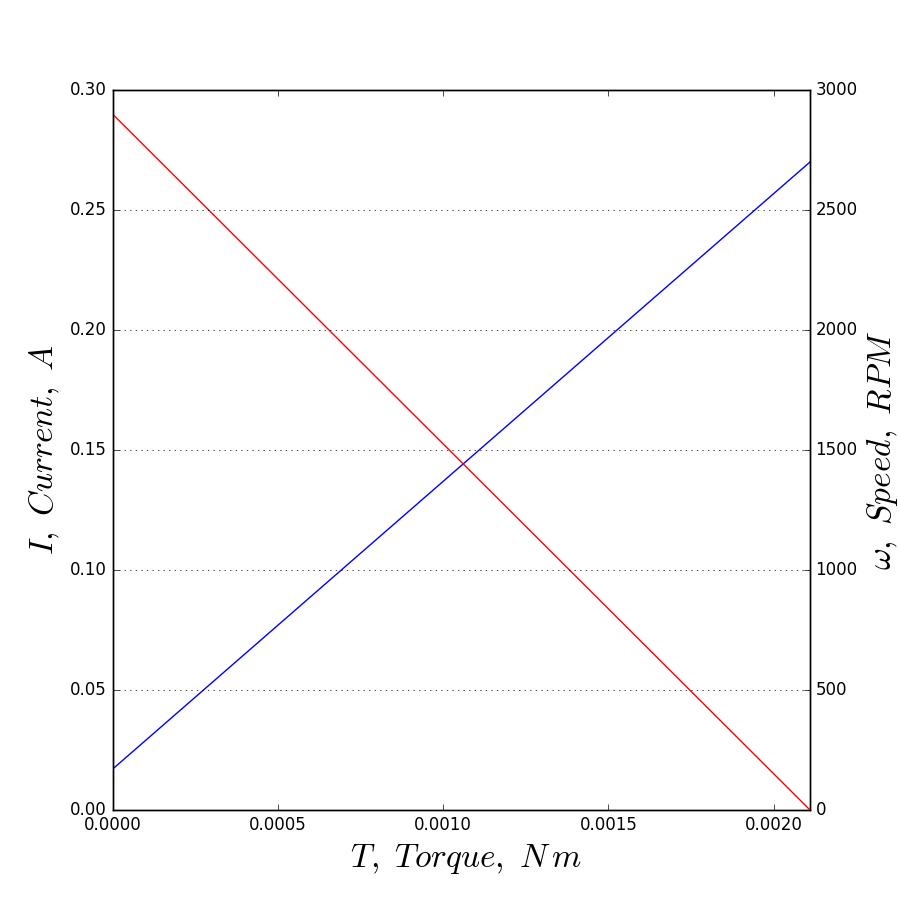
\includegraphics[scale=0.35]{figures/fig_mot_char_example.png}
		\caption{Example DC Motor Characteristic Curve (adapted from \cite{dvdmotordat})}
		\label{figmotcharexample}
		\begin{subfigure}{0.9\textwidth}
			\footnotesize Motor current draw plotted against torque load (blue line) and motor rotational speed plotted against torque (red line).
		\end{subfigure}
	\end{figure}
	
	\section*{Raspberry Pi}
	It was noticed that people were not properly learning about how computers work in schools and universities and so a team of academics at the University of Cambridge created the Raspberry Pi Foundation, and developed the Raspberry Pi Model A as a platform to facilitate education \cite{pihistory}. The Raspberry Pi is a small (85\,mm x 56\,mm \cite{pi3mechdraw}) computer. By default, it runs a version of GNU/Linux called ``Raspbian". There are a number of alternative operating systems suitable for different applications (media center, embedded smart technology) \cite{piotheros}.  \newline
	\begin{figure}[!htb]
		\centering
		\includegraphics[scale=0.3]{images/annotpidia.png} %https://www.draw.io/#Hcbosoft%2Fpi_rheo_proj%2Fmaster%2Fwrite_up%2Fimages%2Fannot_pi_dia.xml
		\caption{Raspberry Pi 3 Model B (adapted from  \cite{pi3info})}
		\label{pidia}
	\end{figure} 
	\newline
	\noindent
	The first Raspberry Pi (Model A) had a single core 700\,MHz processor and 256\,MB of RAM \cite{pi1info}, while the current Raspberry Pi 3 Model B has a quad core 1.2\,GHz and 1\,GB of RAM (also including built in WiFi and Bluetooth) \cite{pi3info}. 
	\br
	Despite being initially designed for educational purposes, the Raspberry Pi has found success in other areas such as with hobbyists \cite{pihobbynotedu} and in industry \cite{pimorethanedu}. As a research tool, the Raspberry Pi has been used as a miniature server for researching the traffic patterns in data centres (the Pis were emulating the behaviours of full scale servers) \cite{piglasgowdc}.
	\br
	What makes the Raspberry Pi attractive as a process controller are the GPIO pins (General Purpose Input/Output, see Figure \ref{pidia}) made available on the main board, similar to a microcontroller. These pins allow electronic circuits to interface with the Raspberry Pi, and thus software to interact with the real world in a way that is not easy to accomplish with a traditional computer. This marriage of microcontroller and desktop computer allows for development, and testing in a single package. In addition, the Raspberry Pi retails (at the time of writing) for \pounds 30.00 \cite{picost}, making it a very cost effective alternative to other control solutions (which can cost several hundred pounds \cite{otherpcucost}). 
	\br
	The GPIO pins are the heart of the Raspberry Pi. Each pin is numbered so that they can be referenced and distinguished between their functions. Some of the pins on the GPIO header are power pins, some are grounded, most are GPIO pins. Each GPIO pin supports digital signals. Resistors attached to the GPIO pins can be used to ``pull-up" or ``pull-down" the signal. If a pin is pulled down, its signal is normally low - it needs to be actively raised high. If a signal is pulled up, it is normally high - it can be lowered by connecting it to ground, but without that it will try to be high. These pull-up and pull-down resistors are included in the Raspberry Pi internally and are activated/deactivated programmatically.
	
	\begin{figure}[!htb]
		\centering
		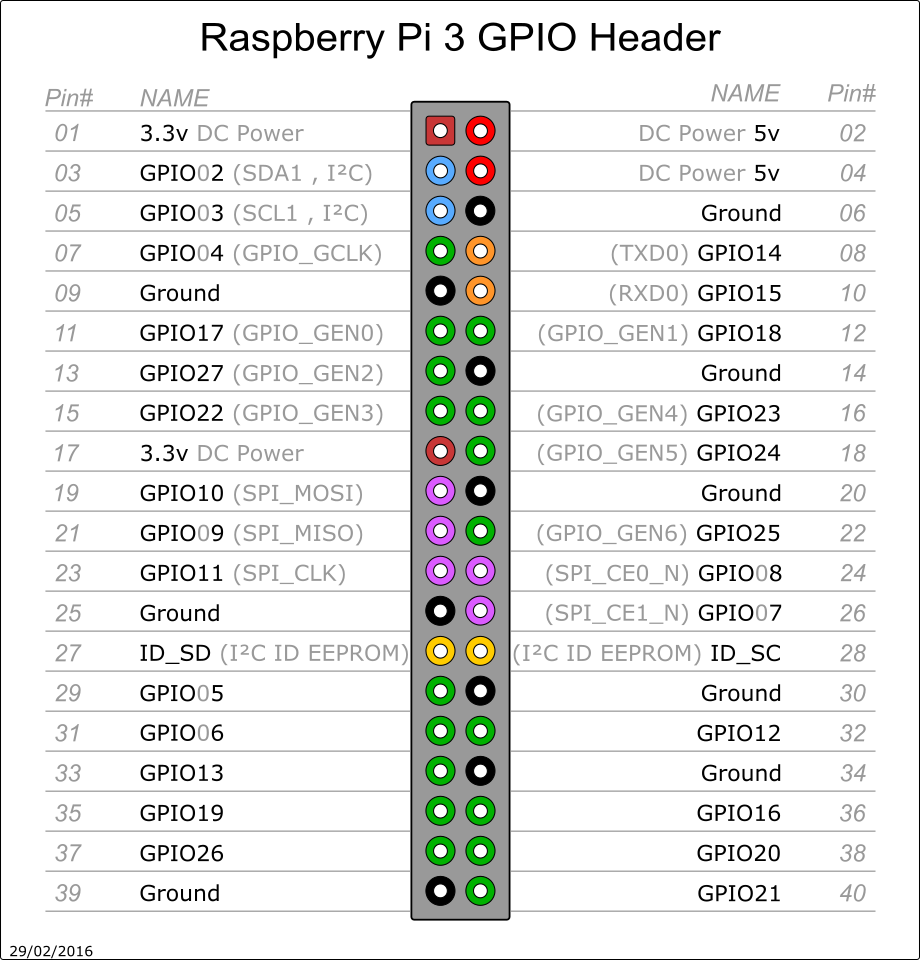
\includegraphics[scale=0.2]{images/gpiopinout.png}
		\caption{Raspberry Pi 3 Model B GPIO Pinout Diagram (taken from  \cite{pigpiopinout})}
		\label{gpiopinout}
	\end{figure}
	
	\noindent
	In addition to simple GPIO functionality, some of the Raspberry Pi's GPIO pins have special functionality, like the ability to use serial communication making inter-device communication much easier. To send the number 1750 to an integrated circuit, the Raspberry Pi would need at least 11 free GPIO pins. While this is not impossible, the number of GPIO pins used for this single action is inconvenient. This can easily be sent via serial connection with just two wires. There are several serial communication options built into the Raspberry Pi: $I^2C$ (Inter-Integrated Circuit) and SPI (Serial Peripheral Interface) are two. SPI uses up to four wires for communication: a clock line for synchronising data transfer, a master-out-slave-in data line (MOSI), a master-in-slave-out (MISO), %not the soup
	and a chip select line for selecting which slave device the master is communicating with.
	
	\section*{Process Control}
	Process control is an important area of process design; the process (whatever it may be) has parameters which must be controlled so that the process continues under the design parameters; at the correct temperature, pressure, etc. Process control has historically been achieved through the use of analogue equipment, using pressurised air to send and receive signals from process equipment. Modern process control is achieved through the use of computers and digital electronics, where the analogue measured signals are converted into digital signals, so that a computer can understand the data. The controller applies an algorithm to calculate the control action required to maintain the desired value of the variable. The modern digital controller can deal with almost any form of input, guarding against a wide variety of disturbances. If it can be measured, it can be controlled.
	\br
	At the heart of the modern controller is the control algorithm. This is the calculation which determines what change to the control output needs to be made (the control action). Control algorithms vary with application. The most commonly used algorithm is the Proportional-Integral-Derivative algorithm (PID control), consisting of three sections which can be turned off or on depending on the needs of the situation:
	\begin{itemize}
		\item Proportional control increases the control action proportional to the size of the error (the difference between the set point and the measured value). This is easy to tune and set up, however it suffers from offset bias. This bias arise from the control action being balanced out in the process by the error such that the control action is not sufficient to change the process to compensate for the error. The error will remain, and the controller will do no more to correct for it, thus an offset is sustained. This must be manually corrected for.
		\item Integral control increases the control action depending on the integral of the error with respect to time (the longer the error goes on, the higher the control action). Integral action is useful to eliminate the offset bias of proportional control.
		\item Finally, derivative control increases control action with the derivative of the error with respect to time, so a quickly rising error is met with a large change in control action. Derivative action is difficult to tune and highly sensitive to noise in the circuit - this means it is rarely used. If it is used, it requires some form of noise filter on the signal and careful tuning. The most common version of the PID algorithm only uses proportional and integral action (no derivative) - the PI controller. PI control allows for easy tuning and quick response, without the difficulties of derivative action, or the offset bias of proportional control.
	\end{itemize}
	Each control element has an associated gain parameter which affects how strongly that element is represented in the control action. These parameters must be set properly before controller can be used. This is done in a process called tuning. There are a variety of methods for tuning the controller, most commonly used is the Ziegler-Nichols method, involving tuning the controller such that the measured value oscillates in a sustained way. Then using the period of oscillation along with other measured parameters to decide on the optimum controller tuning. After tuning using a method such as Ziegler-Nichols it is often required to tweak the tuning manually to obtain the most effective controller for the situation. This is done mostly by trial and error. Trial and error tuning can also be used to fully tune the device, although this would take a long time to do by hand.
	
	\subsection*{Noise Filter}
	Data read by sensors from the real world is often noisy: it will rarely be a single value. Instead, the signal will vary between values around the actual value. This varying of the signal is called noise. Noise can originate from many sources: power supply variations, temperature, or even air pressure. Some noise can be easily predicted and identified (e.g. a 50\,Hz noise waveform in the signal is probably due to the power supply) but others cannot be so easily predicted. 
	\br
	Filtering techniques can be used to eliminate noise from a signal. Frequency filters remove certain frequencies from the signal. Other filtering techniques include: fitting polynomial equations to sections of the data (``splines") - a more graphical method of removing the noise; using a probabilistic analysis of the data to determine the main response; or using a moving average of the data (which can be weighted to favour the data surrounding the current point being filtered).
	\br
	Another set of filtering algorithms are frequency filters which remove the parts of the signal which have a frequency or range of frequencies. High pass filters remove low frequency signals while letting high frequency parts of the signal through. Similarly, low-pass signals maintain low frequency signals and block high frequency signals (like noise). The latter is of particular interest when cleaning noise from a signal. Frequency filtering works by moving the signal into the frequency domain by Fourier transform. Then, a function is applied which drops off to zero very quickly - this selects desired frequencies and removes undesired frequencies. Noise in the signal is high frequency, therefore a low pass filter is desired to allow low frequency signals to pass through (the data) and the high frequency signals (noise) to be eliminated. One such function that can be applied is the Butterworth function (transfer function Equation \ref{eqnbuttgain}). This function is well suited as a frequency filter as it drops of steeply after the cutoff frequency, ensuring most unsuitable parts of the signal are removed \cite{backsignalbutter}. The Butterworth gain transfer function (Equation \ref{eqnbuttgain}) is applied to the frequency domain signal - responding as in Figure \ref{figbutter}.
	
	\begin{figure}[!htb]
		\centering
		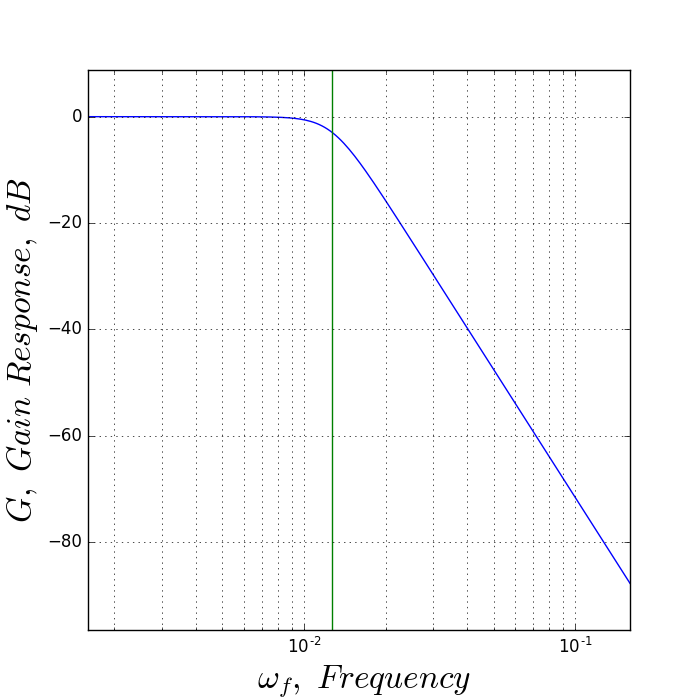
\includegraphics[scale=0.45]{figures/fig_butter.png}
		\caption{Frequency Domain Signal Response To Butterworth Function}
		\label{figbutter}
		\begin{subfigure}{0.8\textwidth}
			\centering
			{\footnotesize 4$^{th}$ order Butterworth filter response (blue line) with 0.0127 Hz cut-off frequency (green line).}
		\end{subfigure}
	\end{figure}
	
	\begin{equation}
	|G(j\omega)| = \frac{1}{\sqrt{1 + \left(\frac{\omega_f}{\omega_{cf}}\right)^{2n}}}
	\label{eqnbuttgain}
	\end{equation}
	
	\nomenclature{$|G(j\omega_f)|$}{Frequence response, or gain\hfill dB}
	\nomenclature{$\omega_f$}{Passed signal frequency\hfill $\rm \left(\pi\ radians\right)/sample$}
	\nomenclature{$\omega_{cf}$}{Signal cutoff frequency\hfill $\rm \left(\pi\ radians\right)/sample$}
	
	\noindent
	
	
	%=====------++++++=====------++++++=====------++++++=====------++++++=====------++++++=====------++++++=====------++++++=====------++++++=====------++++++=====------++++++=====------++++++=====------++++++
	%=====------++++++=====------++++++=====------++++++=====------++++++=====------++++++=====------++++++=====------++++++=====------++++++=====------++++++=====------++++++=====------++++++=====------++++++
	%=====------++++++=====------++++++=====------++++++=====------++++++=====------++++++=====------++++++=====------++++++=====------++++++=====------++++++=====------++++++=====------++++++=====------++++++
	%=====------++++++=====------++++++=====------++++++=====------++++++=====------++++++=====------++++++=====------++++++=====------++++++=====------++++++=====------++++++=====------++++++=====------++++++
	%=====------++++++=====------++++++=====------++++++=====------++++++=====------++++++=====------++++++=====------++++++=====------++++++=====------++++++=====------++++++=====------++++++=====------++++++
	%=====------++++++=====------++++++=====------++++++=====------++++++=====------++++++=====------++++++=====------++++++=====------++++++=====------++++++=====------++++++=====------++++++=====------++++++
	%=====------++++++=====------++++++=====------++++++=====------++++++=====------++++++=====------++++++=====------++++++=====------++++++=====------++++++=====------++++++=====------++++++=====------++++++
	%=====------++++++=====------++++++=====------++++++=====------++++++=====------++++++=====------++++++=====------++++++=====------++++++=====------++++++=====------++++++=====------++++++=====------++++++
	% Sponsoring Organisation
	%\nc{University of Strathclyde}
	%The project was undertaken at the University of Strathclyde, in the Chemical and Process Engineering (CPE) department. The CPE department at Strathclyde is involved in research that cab be split into three main areas \cite{strathresearch}: nanostructured materials, process development and monitoring, and multiscale simulation and theory.
	%\br
	%The University 
	
	%=====------++++++=====------++++++=====------++++++=====------++++++=====------++++++=====------++++++=====------++++++=====------++++++=====------++++++=====------++++++=====------++++++=====------++++++
	%=====------++++++=====------++++++=====------++++++=====------++++++=====------++++++=====------++++++=====------++++++=====------++++++=====------++++++=====------++++++=====------++++++=====------++++++
	%=====------++++++=====------++++++=====------++++++=====------++++++=====------++++++=====------++++++=====------++++++=====------++++++=====------++++++=====------++++++=====------++++++=====------++++++
	%=====------++++++=====------++++++=====------++++++=====------++++++=====------++++++=====------++++++=====------++++++=====------++++++=====------++++++=====------++++++=====------++++++=====------++++++
	%=====------++++++=====------++++++=====------++++++=====------++++++=====------++++++=====------++++++=====------++++++=====------++++++=====------++++++=====------++++++=====------++++++=====------++++++
	%=====------++++++=====------++++++=====------++++++=====------++++++=====------++++++=====------++++++=====------++++++=====------++++++=====------++++++=====------++++++=====------++++++=====------++++++
	%=====------++++++=====------++++++=====------++++++=====------++++++=====------++++++=====------++++++=====------++++++=====------++++++=====------++++++=====------++++++=====------++++++=====------++++++
	%=====------++++++=====------++++++=====------++++++=====------++++++=====------++++++=====------++++++=====------++++++=====------++++++=====------++++++=====------++++++=====------++++++=====------++++++
	% Methodology
	\nc{Methodology}
	This section describes the final design of the rheometer, in several sections. Section 1 (Hardware Setup) describes that main components of the rheometer, the geometry, and the general layout. Section 2 (Electronic Circuits) describes the purpose and function of the circuits developed for the rheometer. Section 3 (Software) describes the available software, what was used, and what was written. Section 4 (Viscosity Calculation) describes how the viscosity was calculated using the information logged from the rheometer. Finally, Section 5 (Calibrations) describes how the hardware and sensor data was calibrated to be able to obtain useful information.
	\section{Hardware Setup}
	The experiment is based around a Couette cell consisting of two concentric cylinders with a fluid in between. The inner cylinder can be rotated by a DC motor (model 970D161) while the outer cylinder is fixed. The motor is controlled by a Raspberry Pi, which sets the rotational speed and reads the torque load on the motor. This is used to calculate the viscosity of the fluid. Motor speed is read in using a secondary motor acting as a dynamo. The dynamo is spun by the inner cylinder motor and produces a voltage proportional to its rotational speed. This voltage is then read in by the Raspberry Pi.
	Figure \ref{expdia} gives a diagram of the set-up, dimensions of the Taylor-Couette cell are summarised in Table \ref{tabcellgeom}.
	\newline
	\begin{figure}[!htb]
		\centering
		\includegraphics[scale=0.3]{images/exp_set_up.png} % https://www.draw.io/#Hcbosoft%2Fpi_rheo_proj%2Fmaster%2Fwrite_up%2Fimages%2Fexp_set_up.xml
		\caption{Diagram of the Experimental Apparatus}
		\label{expdia}
	\end{figure}
	\begin{table}
		\centering
		\caption{Taylor-Couette Cell Geometry}
		\label{tabcellgeom}
		\begin{tabular}{|c|c|}
			\hline
			Reading 						& Value ($\rm mm$) \\
			\hline
			Inner Cylinder, Diameter 		& $30.5 \pm 0.590 \%$\\
			Inner Cyliner, Height 			& $46.8 \pm 0.577 \%$\\
			Outer Cylinder, Inner Diameter 	& $39.1 \pm 1.230 \%$\\
			Outer Cylinder, Outer Diameter 	& $44.2 \pm 0.476 \%$\\
			Outer Cyliner, Height 			& $39.8 \pm 1.410 \%$\\
			\hline
		\end{tabular}
	\end{table}
	\br
	The outer cylinder is made of glass and is attached to a metal base with epoxy. The metal base of the cylinder is clamped in place on the top plate of a scissor lift - allowing for easy loading and unloading of samples in the rheometer. The inner cylinder is a perspex cylinder built onto the shaft of the motor. The motor, holding the inner cylinder, is held in place by a clamp stand. This clamp stand also holds the dynamo in position.
	\br
	The electronic circuits were built onto a breadboard, which allowed for quick alterations to be made to the circuitry during development, with requiring soldering. Wires connect the electronics to the motor, dynamo, and the power source. A ribbon cable connects the full 40 GPIO pins from the Raspberry Pi to the breadboard circuitry.
	
	\section{Electronic Circuits} % last edited 21/3/2017
	%in depth description of relevant electronic circuits
	Figure \ref{circfull} is a schematic of the entire electronic circuit. The circuit can be split into two sections: the first consists of an analogue to digital converter and the sensor components, and the second consists of the potentiometer and various driver components required to set the motor's supply voltage.
	\begin{figure}[!htb]
		\centering
		\includegraphics[scale=0.3]{images/circfull.png}
		%https://www.draw.io/#Hcbosoft%2Fpi_rheo_proj%2Fmaster%2Fwrite_up%2Fimages%2Fcircfull.xml
		\caption{Schematic Diagram of Electronic Circuits}
		\label{circfull}
	\end{figure}
	
	\subsection*{\textit{Sensor Input}} % last edited 21/3/2017
	%Dynamo
	The speed of the motor was gauged using a second motor acting as a dynamo. The dynamo motor was linked to the first motor by a belt and pulley system. The dynamo motor produces a voltage proportional to the speed it is spun at. This sensor therefore provides a qualitative indication of the speed. A pulley was attached to the dynamo, and a rubber belt was used to transfer rotation from the inner cylinder of the Couette cell to the dynamo. The output from the dynamo was fed into an ADC (MCP3008). The ADC works by comparing an input voltage to a reference voltage. Here, the reference voltage was a 3.3\,V line direct from the Raspberry Pi. This was chosen as it is regulated by the Raspberry Pi and should remain constant thus limiting error in the ADC measurements. The output signal from the ADC is a number between 0 and 1023 (a 10-bit binary number) scaled depending on the input voltage and the reference voltage, and rounded to the nearest integer. See Equation \ref{eqnadc}.
	
	\begin{equation}
	S_{10} \approx 1023 \times \frac{V_{ADCin}}{V_{ref}}
	\label{eqnadc}
	\end{equation}
	
	\nomenclature{$S_{10}$}{ADC 10 bit output signal\hfill --}
	\nomenclature[aV  ]{$V_{ADCin}$}{ADC input voltage\hfill $\rm V$}
	\nomenclature[aV  ]{$V_{ref}$}{ADC reference voltage\hfill $\rm V$}
	
	\noindent
	The dynamo speed sensor was the final choice after two other methods were attempted. A Hall effect sensor was used to detect the presence of a magnet attached to the inner cylinder. This was set up such that the Raspberry Pi could (via the HES) calculate the number of rotations in a given time period, or measure the length of time in the gap between rotations. A similar method used a light gate (a UV LED and a phototransistor) and a mask attached to the inner cylinder. As the cylinder rotates, the mask blocks the UV light from shining on the phototransistor and thus the transistor blocks the flow of electrons between its gate and source pins - which can be detected by the Raspberry Pi. Issues arose, however, with the Raspberry Pi's ability to measure time accurately. This is because the python environment is not well suited to accurately reporting time due to the memory management processes enacted by python and even the underlying Linux kernel in the operating system \cite{backrpibadrealtime}. This lead to the dynamo qualitative speed sensor to be used in favour of the quantitative speed sensors due to its ease of use and reliability.
	\br
	To sense the current drawn by the motor, a Hall Effect Current Sensor, or HECS (ACS712, 30\,A sensing range) is used. A Hall effect sensor produces a voltage proportional to the strength of a magnetic field which is produced by running a current through a coil with a magnetically permeable core. The sensor package contains both the coil and the hall effect sensor such that when a current is passed between the sensor pins, a voltage proportional to this current is produced across the output pins. The normal output (at zero amps sensed) is half of the supply voltage of 5\,V. The direction of the current will determine whether the voltage will increase above 2.5\,V or decrease below 5\,V. The current draw by the motor will only ever be in a single direction, so the directional information is unnecessary. Due to the large possible range of the device (being able to sense from -30\,A to +30\,A), the voltage will be boosted to allow the ADC to see a better range of values. In addition, the direction information is removed by subtracting 2.5\,V. The signal is then amplified by 10 and fed into the ADC. 
	\br
	To reduce noise in the HECS reading, a further two sensors (both ACS712s, 5\,A sensing range) were used together with the original sensor. The second and third sensors had a smaller sensing range, which was better suited to this application and they did not require boosting to improve the resolution of the signal. The data from the three sensors is averaged together in data processing to provide a more reliable signal.
	
	\subsection*{\textit{Motor Speed Control}} % last edited 21/3/2017
	The speed of the motor is controlled by altering the supply voltage to the motor. A higher supply voltage, a higher rotational speed. The Raspberry Pi sends a digital serial signal (using the SPI protocol) to a digital potentiometer (MCP4131) which then sets its wiper resistance accordingly. The potentiometer is part of a voltage divider, the output voltage of which varies with the potentiometers resistance and therefore can be controlled by the Raspberry Pi.
	\br
	Within the potentiometer: \(R_{AW}\) is the resistance between terminal A and the wiper pin, and \(R_{WB}\) is the resistance between the wiper and terminal B. The data sent to the potentiometer determines the values of \(R_{AW}\) and \(R_{WB}\), which will total a constant value: \(R_{pot} = 10\,{\rm k\Omega} \). The digital potentiometer is used in a voltage divider configuration, which allows the voltage in a parallel circuit to be controlled. When the resistance is changed to a new value, the voltage across the motor will change according to Equation \ref{eqnvoldiv}. Resistor \(R_2\) is used to set the minimum output voltage. At \(R_2 = 0\,{\rm\Omega}\), the output would vary between 0\,V and 5\,V. While this would also be useful, it limits the resolution of the potentiometer as the bottom volt of this range will not be able to sufficiently power the motor. To bring this minimum up (and thus be able to utilise more of the potentiometer) \(R_2\) is set at \(3\,{\rm k\Omega} \). The digital potentiometer can only handle voltages up to 5\,V across its terminals, an amplifier (gain = 2.1) is used to boost the voltage range from 1.2\,V to 5\,V up to 2.52\,V to 10.5\,V. A transistor (BD243C) is used to boost the current output from the amplifier, which can only supply around 20\,mA. The transistor boosts this up to 2\,A (hFE = 100).
	\begin{equation}
	V_{out} = V_{in}\times \frac{R_2 + R_{WB}}{R_2 + R_{pot}}
	\label{eqnvoldiv}
	\end{equation}
	\begin{equation}
	V_{min} = V_{in}\times \frac{R_2}{R_2 + R_{pot}}
	\label{eqnminvol}
	\end{equation}
	\begin{equation}
	V_{max} = V_{in}\times \frac{R_2 + R_{pot}}{R_2 + R_{pot}} = V_{in}
	\label{eqnmaxvol}
	\end{equation}
	
	\nomenclature[aV ]{$V_{out}$}{Voltage output \hfill $\rm V$}
	\nomenclature[aV ]{$V_{in}$}{Voltage input \hfill $\rm V$}
	\nomenclature{$R_{AW}$}{Resistance between potentiometer wiper and A terminal\hfill $\rm \Omega$}
	\nomenclature{$R_{WB}$}{Resistance between potentiometer terminal B and wiper\hfill $\rm \Omega$}
	\nomenclature{$R_{pot}$}{Resistance between terminals A and B on the potentiometer\hfill $\rm \Omega$}
	\nomenclature{$R_{AW}$}{Resistance value ofthe resistor between B terminal on the potentiometer and ground\hfill $\rm \Omega$}
	
	\noindent
	The Raspberry Pi sets the motor speed by setting the resistance in the digital potentiometer. The Pi sends a 7-bit digital signal to the pot, indicating the resistance desired. Within the potentiometer is a network of resistors, and this number will determine the path taken through the circuit, the higher the number, the higher \(R_{WB}\) will be. When this increases, the voltage across the bottom resistor will decrease and the voltage across the motor will mirror this therefore increasing the motor's speed.
	\br
	A 7-bit number has a maximum value of 127 ($2^7 - 1 = 127$). Therefore the potentiometer terminal B-wiper resistance will increase by $78.7\,\rm \Omega$ given a unit increment in potentiometer value (Equation \ref{eqnpotres}). Combining this with Equation \ref{eqnvoldiv} gives an equation for motor supply voltage (also knowing the gain of the operational amplifier circuit) - Equation \ref{eqnmotsupvol}.
	
	\begin{equation}
	V_{wiper} = V_{AB}\times \frac{3{\,\rm k\Omega} + \left(78.7{\,\rm\Omega} \times pv\right)}{13{\,\rm k\Omega}}
	\label{eqnpotres}
	\end{equation}
	
	\nomenclature[aV ]{$V_{wiper}$}{Voltage level at the digital potentiometer output \hfill $\rm V$}
	\nomenclature[aV ]{$V_{AB}$}{Voltage across the potentiometer terminals\hfill $\rm V$}
	
	\begin{equation}
	V_{ms} = 0.0636\, {\rm V} \times pv + 2.423\, {\rm V}
	\label{eqnmotsupvol}
	\end{equation}
	
	\nomenclature[aV ]{$V_{ms}$}{Motor supply voltage\hfill $\rm V$}
	
	%=====------++++++=====------++++++=====------++++++=====------++++++=====------++++++=====------++++++=====------++++++=====------++++++=====------++++++=====------++++++=====------++++++=====------++++++
	%=====------++++++=====------++++++=====------++++++=====------++++++=====------++++++=====------++++++=====------++++++=====------++++++=====------++++++=====------++++++=====------++++++=====------++++++
	\section{Software}
	The Raspberry Pi runs a version of GNU/Linux called ``Raspbian" - specially developed for the Raspberry Pi's ARM Processor. Raspbian is a desktop operating system, and can perform all of the tasks a full size computer can (text processing, internet browsing, etc.). This presents one of the main features of the Raspberry Pi - it can be both development station and testbed. Software was written to enable the Raspberry Pi to communicate with the hardware using the Python language. Python was chosen as it is a very popular, easy to use, and easy to read language (there are rules about how python should be properly written in order to maintain easy-to-read code \cite{pep8ref}). Its popularity means that there is an abundance of software packages available for inclusion. 
	\br
	Packages used here:
	\begin{itemize}
		\item \texttt{RPi.GPIO} \cite{citerpigpio}: comes pre-installed on Raspian and was used for accessing the GPIO pins from a Python environment.
		\item \texttt{spidev} \cite{srcspidev}: used to communicate with devices in an electric circuit using the Serial Peripheral Interface (SPI) protocol.
		\item \texttt{numpy} \cite{numpyref}: used to perform calculations efficiently in the python environment and to fit equations to empirical data (using the \texttt{numpy.polyfit} function).
		\item \texttt{scipy} \cite{scipyref}: used to perform scientific manipulations of data. Primarily used in this project to filter data using functions from the \texttt{scipy.optimise} package.
		\item \texttt{pandas} \cite{pandasref}: used to read Comma Separated Value (\texttt{.CSV}) files - the file format used to log data from experiments.
	\end{itemize}
	
	\begin{figure}[!htb]
		\centering
		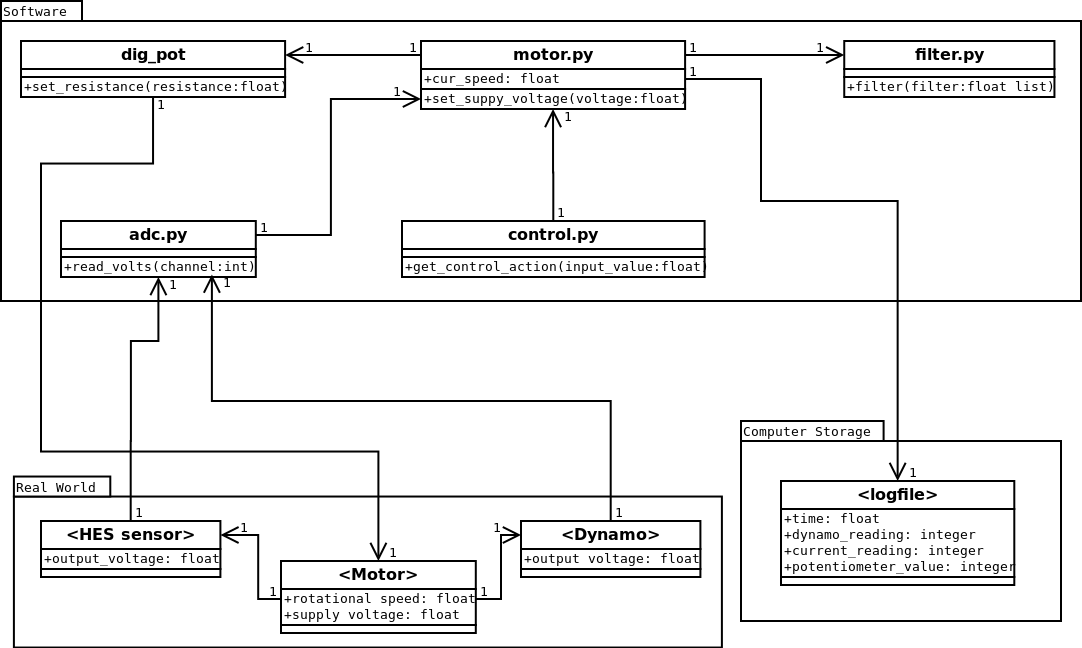
\includegraphics[scale=0.35]{images/codemap.png}
		%RE DO, SOFTWARE WAS SHUFFLED A BIT?
		\caption{Class Diagram}
		\label{figcladia}
	\end{figure}
	
	\noindent
	The software is organised into different classes (see Figure \ref{figcladia}):
	\begin{itemize}
		\item Digital Potentiometer \newline 
		This class manages the sending of data to a digital potentiometer and keeps a record of some key data.
		\item ADC \newline 
		This class manages the sending and receiving of data between the Raspberry Pi and the ADC.
		\item Control\newline 
		This class is a discrete time implementation of the PID algorithm used in process control.
		\item Motor \newline
		This class makes use of the digital potentiometer class to control the voltage supplied to the motor, the ADC class to read in the speed of the motor and the current drawn by the motor. This data is logged at a set rate to be used in calculating the viscosity.
		\item Noise Filter \newline
		A collection of functions that can be used to reduce noise in read data.
	\end{itemize}
	Full copies of the software source code can be found in Appendix 1.
	
	\subsection*{Digital Potentiometer} % last edited 13/3/2017
	This class enables the software to interact with the digital potentiometer (model MCP4131) using the SPI protocol. This class makes use of the \texttt{spidev} package to enable SPI communication. The class contains a function to set a value on the resistor (as an integer number between 0 and 127), and is set up such that multiple digital potentiometers can be included on the same circuit.
	\br
	The class is used, as with all normal classes, by first creating an instance of a class object, passing along the initialisation parameters. These parameters are set in the source code as the parameters to the ``\texttt{\_\_init\_\_}" function. For this class, there is only one initialisation parameter: ``\texttt{chip\_select}", an optional parameter which tells the spidev package which SPI device to talk to. This parameter is 0 by default, but can be changed if the class is used in a different instance to manage another digital potentiometer.
	\br
	To set the potentiometer resistance, a value between 0 and 127 (inclusive) is sent to the potentiometer using the ``\texttt{set\_resistance}" function. This function only requires one parameter - the value to be sent. The spidev package is used to send this value to the correct register on the potentiometer, causing it to alter its resistance.
	
	\subsection*{ADC} % last edited 13/3/2017
	The ADC class enables the software to interact with the analogue to digital converter (both model MCP3008) via the SPI protocol. As with the digital potentiometer, this class makes use of the spidev package. \br
	The initialisation function for the ADC class has two parameters, both optional. The first is a chip select parameter (used to tell spidev which device we are trying to communicate with on the SPI network) which has a value of 1 by default. The second parameter is the value of the reference voltage (\texttt{vref}), 3.3 by default, used to calculate the voltage read in by the ADC from the 10-bit value read from the ADC. \br
	Usage of the class is very simple: the ``\texttt{read\_data}" function returns the value read from the ADC (a 10-bit number) and takes only 1 parameter (a value from 0 to 7 indicating the channel on the ADC to read from). Further, the ``\texttt{read\_volts}" function will read from the ADC and convert the result to a voltage. This function takes a channel indication parameter.
	
	\subsection*{Control} % last edited 13/3/2017
	This class is a discrete-time implementation of a PI controller based upon the PID algorithm (Equation \ref{eqnpidalg}). Due to the random fluctuations in speed caused by the jamming effect, derivative control is not included because derivative action works on the rate of change of the error, therefore a sudden change in the error is going to elicit an extreme response from  the controller which will upset the process. In addition, there will be noise inherent in the signal (discussed in the next section) which will severely impair the controller if derivative action is turned on. 
	
	\begin{equation}
	ca = \pm K_C \left(e + \frac{1}{\tau _I} \int e \space dt + \tau _D \frac{de}{dt}\right)
	\label{eqnpidalg}
	\end{equation}
	
	\nomenclature{$K_C$}{Controller gain\hfill--}
	\nomenclature[g]{$e$}{Error between the set point and controller input\hfill--}
	\nomenclature[g]{$\tau_I$}{Integral time constant\hfill--}
	\nomenclature[g]{$\tau_D$}{Derivative time constant\hfill--}
	\nomenclature{$K_P$}{Proportional action gain\hfill--}
	\nomenclature{$K_I$}{Integral action gain\hfill--}
	\nomenclature{$K_D$}{Derivative action gain\hfill--}
	
	\noindent
	The control class uses a discrete time transfer function of the controller algorithm, formed by first removing the derivative action and taking a Laplace transform. In Laplace domain notation; $U(s)$ or $ca(s)$ is the controller output, and $e(s)$ is the error between the process output (controlled variable) and the set point. The resulting transfer function is shown as Equation \ref{eqnpitf}.
	
	\begin{equation}
	\frac{ca}{e}(s) = \frac{K_P  s + K_I}{s}
	\label{eqnpitf}
	\end{equation}
	
	\noindent
	This class makes use of the \texttt{scipy.signal} package to deal with transfer functions.\br
	The initialisation function for this class has three arguments, described below. Included in the descrption is the data type the function is expecting, and the default value (if applicable).
	
	\begin{itemize}
		\item \texttt{tuning} - tuple (float, float). Represents the proportional and integral gains respectively.
		\item \texttt{set\_point} - float. Optional. The desired value for the controlled process variable. 0 by default.
		\item \texttt{sample\_time} - float. Optional. The interval time between control action updates. By default, this is automatically calculated, but can be set manually here for simulating the response.
	\end{itemize}
	
	Function ``\texttt{get\_control\_action(Y)}" is used to obtain the control action in response to the input. This function takes a single argument: the process output. Then the \texttt{scipy.signal} package's transfer function class is used to obtain the result from the controller's transfer function, giving a suitable control action.
	\br
	For the controller to be useful, it needs to be tuned. This can be done using a modelled transfer function of the process, such as a First Order Plus Dead-Time (FOPDT) model. Using a model, the controller can be simulated to view how it reacts to different tunings. The class includes a simulation function (``\texttt{do\_sim}") to allow for manual tuning. The function uses a transfer function for the process (a first order model) and simulates process output for a length of time after a step change in set point. The results give an indication of how well the controller can manage the process. 
	\br
	There are a number of techniques used to tune controllers, as discussed in chapter 1. Any filtering method used, almost always ends in manual fine-tuning of the results. To speed this process up, a function was written in the control class which iterates through a range of different tunings and decides upon an optimal set. A first order transfer function modelling the process is used in the form of its two main parameters: $\rm\tau_C$, the time constant, and $\rm SSG$, the steady state gain. The time constant gives an indication of the strength of the dynamics of the response, while steady state gain indicates the final value of the response with respect to the given input --- it is the gain after the system has come to steady state. From this model, the process' controlled response is monitored over a simulated minute. The shape of this response is examined to evaluate is optimality (how fast it rises, how much it optimises). This resulting tuning is, as with many other techniques, a starting point for manual fine-tuning. This fine tuning is done by trial and error.
	
	\nomenclature{$\rm\tau_C$}{Time constant of a 1$\rm ^{st}$ order process model transfer function\hfill--}
	\nomenclature{$\rm SSG$}{Steady state gain of a 1$\rm ^{st}$ order process model transfer function\hfill--}
	
	\subsection*{Filter}
	The \texttt{filter} function was written to remove noise from the signal. There is a function in the \texttt{scipy.signal} library which creates a Butterworth filter transfer function, and another used to apply the created filter. This was packaged together within the \texttt{filter.py} package. This function takes in noisy data, applies the filter, and outputs the clean signal. 
	\br
	The Butterworth function in scipy has two parameters: \texttt{N} and \texttt{Wn}. \texttt{N} (n in Equation \ref{eqnbuttgain}) is the order of the Butterworth function, representing how sharply it removes frequencies above the cut-off frequency. \texttt{Wn} is the cutoff frequency normalised against the signal's Nyquist frequency. The Nyquist frequency is the slowest the sample can be sample without causing issues to arise in the read data (like aliasing: signals appearing to move in one way but actually moving in another, like car wheels in low-framerate videos) and is equal to twice the fastest moving dynamics in the signal. By trial and error, the optimal parameters of the filter function were found to be \texttt{N}$ = 2$ and \texttt{Wn} $ = 0.001$. This represents a butterworth function of order 2 with a cutoff frequency one five-hundredth of the highest frequency data in the signal.
	
	\subsection*{Motor}
	This class uses the ADC class to read in the speed of, and current supplied to motor. The digital potentiometer class is used to control the voltage supply to the motor as well. The overall goal of the motor class is to manage every aspect of the motor, and to record as much relevant data as possible. 
	\br
	The class is initialised with several optional variables; most are used by the motor class itself while some are for setting up the ADC class, and some are for setting up the digital potentiometer.
	\br
	Motor-relevant arguments:
	\begin{itemize}
		\item \texttt{startnow} - a boolean value indicating whether the speed poll thread should begin when the class is first instantiated. \texttt{False} by default.
		\item \texttt{poll\_logging} - a boolean value indicating whether data should be logged by the motor to file. \texttt{True} by default.
		\item \texttt{log\_dir} - string, path to directory where the logged data will be saved.
		\item \texttt{i\_poll\_rate} - ``inverse poll rate", the interval between speed polls. A higher value results in sporadic data and lower processing requirements, a low value results in better data but a higher toll on the Raspberry Pi's resources. \texttt{0.1} by default.
		\item \texttt{svf} - ``speed-voltage-function", tuple representing the two coefficients in a linear fit equation for the relationship between the motor's rotational speed and the voltage reading in from the dynamo via the ADC. \texttt{(312.806, -159.196)} by default.
	\end{itemize}
	The motor class can be used to set the supply to a motor (using a digital potentiometer), can read in the motor's speed and calculate its current draw (using the ADC).
	
	
	%=====------++++++=====------++++++=====------++++++=====------++++++=====------++++++=====------++++++=====------++++++=====------++++++=====------++++++=====------++++++=====------++++++=====------++++++
	%=====------++++++=====------++++++=====------++++++=====------++++++=====------++++++=====------++++++=====------++++++=====------++++++=====------++++++=====------++++++=====------++++++=====------++++++
	\section{Viscosity Calculation}
	\subsection*{Calculated Method}
	The viscosity of a fluid can be calculated using Newton's Viscosity Law, Equation \ref{eqnvisco}:
	\[\mu = \frac{\tau}{\dot{\gamma}}\]
	\newline
	The shear stress and strain rate can be calculated from calibrated data from the motor, as well as speed and current supply readings from sensors. From a characteristic curve for a motor (Figure \ref{figmotcharexample}), Equations \ref{eqnmotcharI_obfs} \& \ref{eqnmotcharO_obfs} were read.
	
	\begin{equation}
		I_{ms} = I_{emf} \times \frac{T}{T_S} + I_{coil}
		\label{eqnmotcharI_obfs}
	\end{equation}
	\begin{equation}
		\omega = \omega_N \times \left(1 - \frac{T}{T_S}\right)
		\label{eqnmotcharO_obfs}
	\end{equation}
	
	\noindent
	Both $I_{emf}$ and $I_{coil}$, as well as the stall torque $T_S$, vary with voltage supplied to the motor ($V_{ms}$) and calibrations were obtained for coil current as a function of supply voltage($I_{coil} (_{V_{ms}})$) and EMF current divided by stall torque as a function of supply voltage ($\frac{I_{emf}}{T_S} (_{V_{ms}})$): Equations \ref{eqnemftscalea} \& \ref{eqnicocalea}). The supply current is measured, and the supply voltage is controlled, the motor torque can then be calculated using Equation \ref{eqntorqueget}.

	\begin{equation}
		T = \frac{I_{ms} - I_{coil} (_{V_{ms}})}{\frac{I_{emf}}{T_S} (_{V_{ms}})}
		\label{eqntorqueget}
	\end{equation}
	\begin{equation}
		I_{coil} (_{V_{ms}}) = A_{Icoil} \times V_{ms} + B_{Icoil}
		\label{eqnicocalea}
	\end{equation}
	\begin{equation}
		\frac{I_{emf}}{T_S} (_{V_{ms}}) = A_{IemfTs} \times V_{ms} + B_{IemfTs}
		\label{eqnemftscalea}
	\end{equation}
	
	\nomenclature{$I_{coil}$}{Current drawn due to resistance in motor coils\hfill $\rm A$}
	\nomenclature{$I_{emf}$}{Current drawn due to motor loading\hfill $\rm A$}
	\nomenclature{$A_{Icoil}$}{Coefficient in coil current calibration\hfill $\rm A\,V^{-1}$}
	\nomenclature{$B_{Icoil}$}{Y-intercept in coil current calibration\hfill $\rm A$}
	\nomenclature{$A_{IemfTs}$}{Coefficient in emf current/stall torque calibration\hfill $\rm A\,Nm^{-1}\,V^{-1}$}
	\nomenclature{$B_{IemfTs}$}{Y-intercept in emf current/stall torque calibration\hfill $\rm A\,Nm^{-1}$}
	
	Torque is a force acting rotationally from a point source through a length. This length, in this case, is the radius of the inner cylinder of the Taylor-Couette cell. The torque is divided by this length, giving the force applied by the motor. This is the force applied to the fluid which causes the shear: the area over which this is applied is used to obtain the shear stress applied to the fluid (Equation \ref{eqntaut}).
	
	\begin{equation}
	\tau = \frac{T}{2 \times \pi \times r_i^2 \times H}
	\label{eqntaut}
	\end{equation}
	
	\nomenclature{$\tau$}{Shear stress\hfill $\rm Pa$}
	\nomenclature{$H$}{Fill depth of the Taylor-Couette cell\hfill $\rm m$}
	
	\noindent
	The strain rate imposed upon the fluid in the gap between the cylinders can be calculated using Equation \ref{eqnavsr}. The strain rate is the derivative of the velocity of the fluid in the gap. If the velocity varies linearly through the gap (as in ideal Couette flow), then the derivative will simply be the velocity ($ms^{-1}$) divided by the gap size ($m$) \cite{couetteshearcell}.
	\begin{equation}
	\dot{\gamma} = \frac{\omega r_i}{r_o - r_i}
	\label{eqnavsr}
	\end{equation}
	
	\nomenclature[g]{$\dot{\gamma}$}{Shear rate\hfill $\rm s^{-1}$}
	\nomenclature{$r_i$}{Inner cylinder radius\hfill $\rm m$}
	\nomenclature{$r_o$}{Outer cylinder radius\hfill $\rm m$}
	
	\subsection*{Calibrated Method}
	A further method for calculating the viscosity was used. The rheometer was calibrated with several reference fluids at a single voltage to obtain an expression for the motor's torque as a function of the supply current. This can then be used in a similar manner to above, using the torque calibration to obtain the viscosity from the current reading and the speed of rotation of the motor.
	\br
	It is known that the motor torque varies with both supply current and supply voltage. By setting the voltage to a single value, the output torque can be calibrated against the current drawn by the motor. This method differs from the previous method in the way the torque is calculated: using Equation \ref{eqntrefcal} rather than Equation \ref{eqntorqueget}.
	\begin{equation}
	T = A_{TI} \times I_{ms} + B_{TI}
	\label{eqntrefcal}
	\end{equation}
	\nomenclature{$A_{TI}$}{Coefficient in torque calibration\hfill $\rm Nm\,A^{-1}$}
	\nomenclature{$B_{TI}$}{Y-intercept in torque calibration\hfill $\rm Nm$}
	%=====------++++++=====------++++++=====------++++++=====------++++++=====------++++++=====------++++++=====------++++++=====------++++++=====------++++++=====------++++++=====------++++++=====------++++++
	%=====------++++++=====------++++++=====------++++++=====------++++++=====------++++++=====------++++++=====------++++++=====------++++++=====------++++++=====------++++++=====------++++++=====------++++++
	\section{Calibrations}
	
	\subsection*{Dynamo Calibration}
	The goal is to find a function of the dynamo output voltage that gives the rotational rate of the motor (i.e. \(\omega ({V_D})\)). To do this, the motor's speed was varied by varying the supply voltage (using the digital potentiometer) to different discrete levels. The \texttt{motor} class was used to perform this so that sensor readings were logged automatically. At each voltage level, the speed was read several times using a contact tachometer to give the actual speed. The dynamo readings were taken from the logs and filtered using the \texttt{filter} package. The clean dynamo data was then compared to the speed readings taken from the tachometer. The \texttt{numpy} package was used to form a first-order empirical relationship between the variables: Equation \ref{eqnspdvvr}. 
	\br
	The digital potentiometer was to give a supply voltages between 2.275 and 10.723, in steps of 0.528. At each supply voltage, A tachometer was used to read the speed (in m/s). The reading was taken five times per supply voltage and the dynamo voltage level was recorded at intervals of 100ms by the Raspberry Pi. The contact tachometer had to be used carefully, it had to make strong enough contact with the cylinder in order to transfer the speed to the tachometer's rotor, but without impacting the speed of the motor and thus obtain an incorrect reading. The average value of each speed reading, and the dynamo voltage readings were plotted on Figure \ref{figspeedvrvolt}.
	
	\begin{equation}
	\omega = 308.768 \times {V_D} - 167.080
	\label{eqnspdvvr}
	\end{equation}
	
	\nomenclature{$v_m$}{Motor rotational speed\hfill $\rm RPM$}
	\nomenclature[aV ]{$V_D$}{Dynamo output voltage\hfill $\rm V$}
	
	\begin{figure}[!htb]
		\centering
		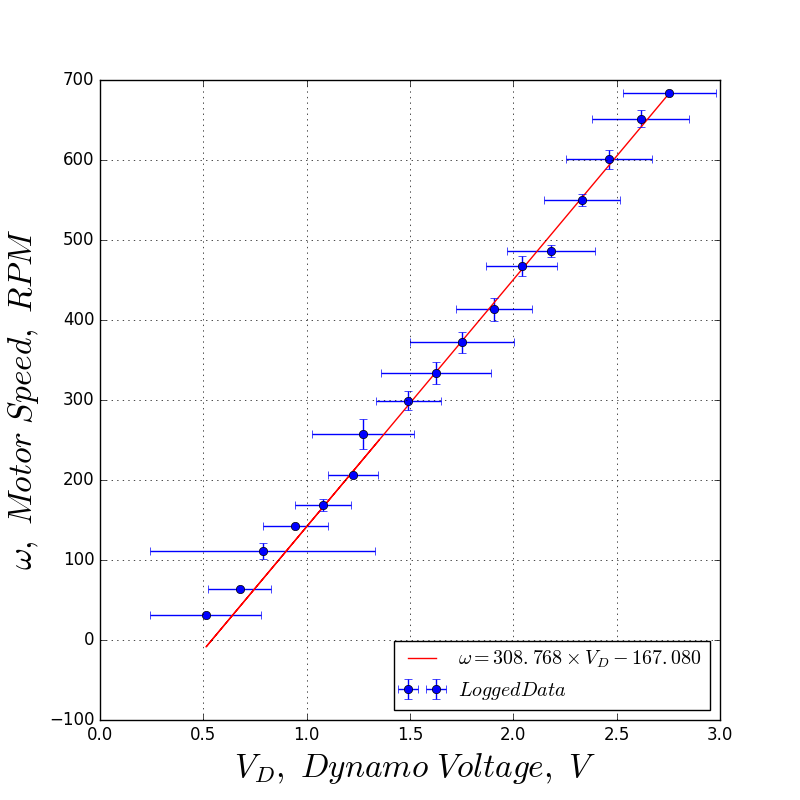
\includegraphics[scale=0.45]{figures/fig_speed_v_rvolt.png}
		\caption{Dynamo Calibration Results}
		\label{figspeedvrvolt}
		\begin{subfigure}{0.9\textwidth}
			\footnotesize Recorded dynamo voltages and corresponding speed in RPM (blue circles). The error bars represent one standard deviation. Also plotted is a line of best fit (red line).
		\end{subfigure}
	\end{figure}
	
	\noindent
	In addition, a relationship between the load-less rotational speed (no-load speed) and the potentiometer value was found, from the same logged data: Equation \ref{eqnsvemp} (see Figure \ref{figdynocheck}).
	
	\begin{equation}
	\omega_{NL} = 5.13 {\rm \, RPM} \times pv + 15.275 {\rm \, RPM}
	\label{eqnsvemp}
	\end{equation}
	
	
	\subsection*{HECS Calibration}
	The goal for this was to find a function of the HECS output voltage reading that gives the current drawn by the motor (i.e. \(I_{ms} ({V_{HES}})\)) for both types of HECS sensor. The current was read at different supply voltages from a multimeter placed in the circuit. The logged data during this run was examined to compare the HECS voltages with the ammeter current reading. The current supply was plotted against the HECS sensor voltages output (see Figures \ref{fighes30a} \& \ref{fighes5a}). A first order equation was fit to the data (using the \texttt{numpy} package) to give Equation \ref{eqnhescal} for the 30A sensor and Equation \ref{eqndualhescal} for the two 5A sensors.
	\begin{equation}
	I_{ms} = 15.93 {\rm \, \frac{A}{V}} \times {V_{HES}} - 28.59 {\rm \, A}
	\label{eqnhescal}
	\end{equation}
	\begin{equation}
	I_{ms} = 3.580 {\rm \, \frac{A}{V}} \times {V_{HES}} - 7.784 {\rm \, A}
	\label{eqndualhescal}
	\end{equation}
	
	\nomenclature{$I_{ms}$}{Motor supply current\hfill $\rm A$}
	\nomenclature{$V_{HES}$}{Hall effect sensor output voltage\hfill $\rm V$}
	
	\noindent
	Where \(I_{ms}\) is the motor supply current, in amps, and \(V_{HES}\) is the voltage output from the Hall Effect Sensor as it enters the ADC, in volts.
	
	\begin{figure}[!htb]
		\centering
		\begin{subfigure}[t]{0.45\textwidth}
			\centering
			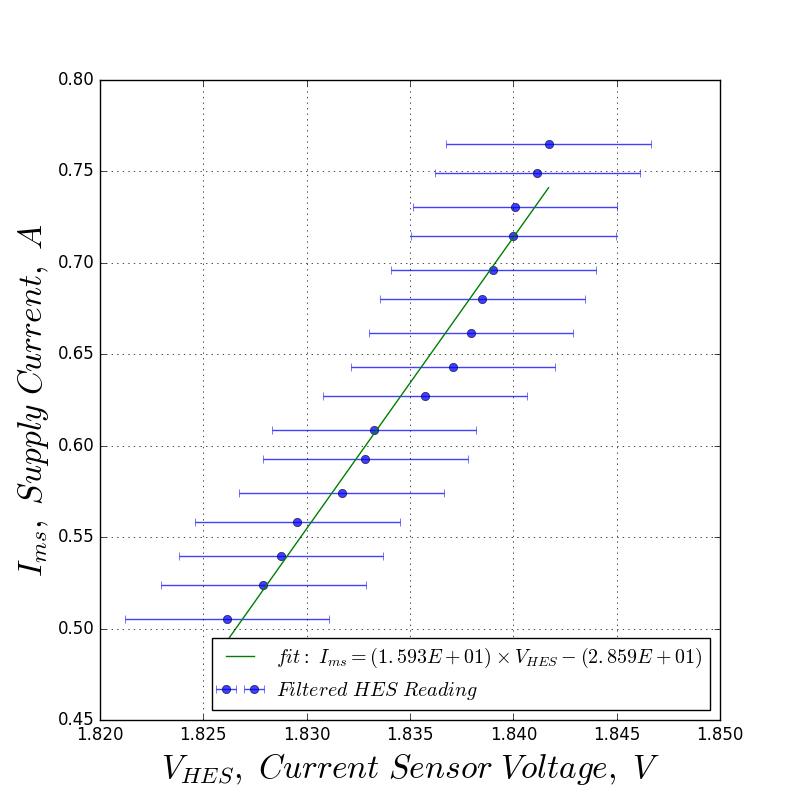
\includegraphics[scale=0.3]{figures/fig_hes_cal.png}
			\caption{30A HECS Calibration}
			\label{fighes30a}
			\footnotesize
			Supply current plotted against the filtered 30A HECS input (blue cirles). Error bars represent one standard deviation in the data. A 1$\rm ^{st}$ order polynomial was fit to the data (green line).
		\end{subfigure}
		\begin{subfigure}[t]{0.45\textwidth}
			\centering
			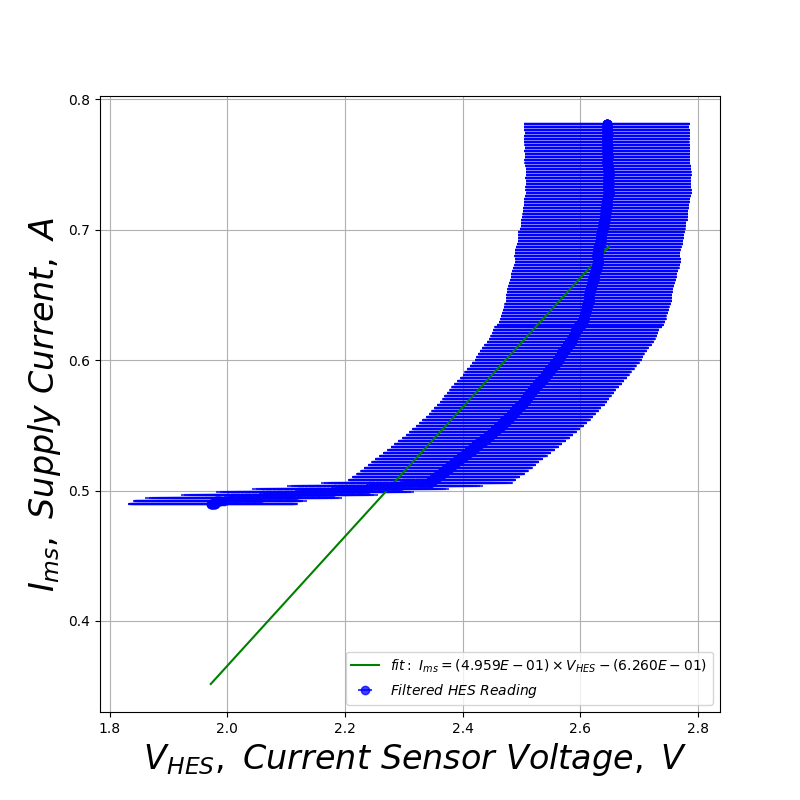
\includegraphics[scale=0.3]{figures/fig_dual_hes_cal.png}
			\caption{Dual 5A HECS Calibration}
			\label{fighes5a}
			\footnotesize
			Supply current plotted against the filtered 5A HECS input (blue cirles). Error bars represent one standard deviation in the data. A 1$\rm ^{st}$ order polynomial was fit to the data (green line).
		\end{subfigure}
		\label{hescalcomp}
		\caption{HECS Calibration Results}
	\end{figure}
	
	\subsection*{Reference Fluid Viscosity}
	A relationship between the motor's torque output and the current drawn by the motor was obtained. This was done by putting a fluid of known viscosity into the rheometer and running it at constant shear rate. With the viscosity known and the strain rate known, the shear stress can be calculated. This shear stress was compared with the current draw and a linear equation was fit. 
	\br
	The compositions of the reference solutions were chosen to give solutions of viscosities evenly spaced between $\mu_{water} = 0.001\rm\,Pa\,s$ and $\mu_{glycerol} = 1.41\rm\,Pa\,s$. This was estimated by using tabulated data \cite{seguroberglycsolvisc}. The temperature in the laboratory is roughly 15$\,\rm^oC$, and so the solutions' viscosity at this temperature was interpolated from data at 10$\,\rm^oC$ and 20$\,\rm^oC$. Table \ref{tabreffluvisc} shows both the theoretical and actual viscosities of the solutions used. 30\,ml of each solution was prepared by measuring out the required volume of glycerol with a syringe (BD Plastic, 5\,ml) and the required water with a micro-pipette (ErgoOne, 20$\,\rm\mu l$ to 200$\,\rm\mu l$) (the pure glycerol solution was far too viscous for the pipette to be able to measure out the volumes accurately). The solutions were split into two containers, one filled up to 20\,ml to be used in the rheometer, and another filled up to 10\,ml to be tested separately by a Discovery Hybrid Rheometer 2 (DHR-2). 
	\br
	The DHR-2 was used to obtain an exact value for the viscosity of the solutions used. A small amount of each solution was tested with the DHR-2's 40\,mm parallel plate head at strain rates from 5$\,\rm s^{-1}$ to 250$\,\rm s^{-1}$. each sample was tested 3 times to confirm the result. The theoretically estimated data and the actual viscosity readings differ slightly. This is likely due to water contamination of the glycerol used to produce the solutions. Glycerol is very hydrophillic and will draw moisture out of the air. The viscosity of a glycerol water solution is highly sensitive to the presence of water (increasing water content from 0.00\% to 11.13\% by volume results in the viscosity dropping by 2.3\,Pa\,s) therefore even a tiny amount of water in the glycerol source fluid is going to alter the viscosity hugely. It would be better to use higher viscosity solutions for a better range of values, but the important thing is that the reference solutions are of accurately known viscosity. 
	\newline
	\begin{table}
		\centering
		\caption{Compositions and Viscosities of Selected Aqueous Glycerol Solutions at 15$\,\rm^oC$}
		\label{tabreffluvisc}
		\begin{tabular}{| c | c | c |}
			\hline
			Composition (vol\% glycerol) & Theoretical Viscosity ($\rm Pa\,s$) & Actual Viscosity ($\rm Pa\,s$)\\
			\hline
			100.0\% & 2.656 & 1.328 \\
			98.73\% & 2.120 & 1.129 \\
			96.23\% & 1.104 & 0.9061 \\
			93.75\% & 0.613 & 0.6102 \\
			88.87\% & 0.358 & 0.4005 \\
			\hline
		\end{tabular}
	\end{table}
	
	\subsection*{Motor Coil Current Calibration}
	This calibration is required to obtain an expression for the coil current in the motor as a function of the supply voltage. To obtain the coefficients for this calibration, the supply voltage to the motor was varied while the current draw was read and logged automatically.
	\begin{equation}
	I_{coil} (V_{ms}) = A_{Icoil} \times V_{ms} + B_{Icoil}
	\label{eqnicocalmid}
	\end{equation}
	
	\begin{figure}[!htb]
		\centering
		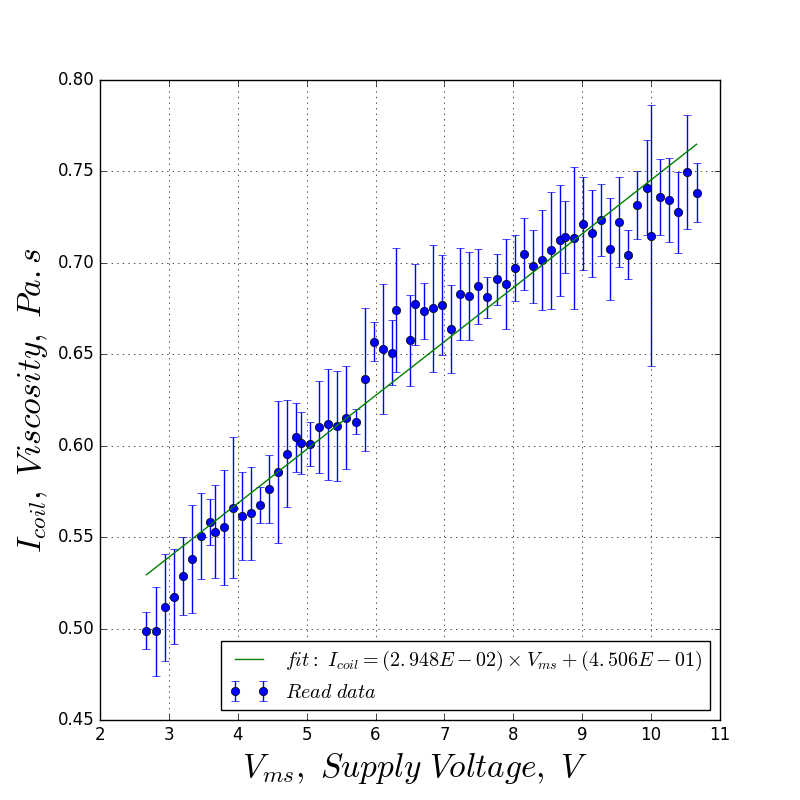
\includegraphics[scale=0.45]{figures/fig_ico_cal.png}
		\caption{Coil Current Calibration Results}
		\label{figicocal}
		\begin{subfigure}{0.9\textwidth}
			\footnotesize 
		\end{subfigure}
	\end{figure}
	
	\noindent
	With no loading on the motor, the measured current is the current through the coil ($I_{coil}$). Therefore, the measured current data can be compared with the supply voltage to obtain the coefficients for the desired calibration. The motor supply voltage was varied over the course of ten minutes between 2.52\,V and 10.5\,V. This was done via a script written for the purpose using the software written previously. The motor class was used both to manage the supply voltage, and to log the current sensor readings. The resulting information was plotted on a graph (Figure \ref{figicocal}) and a linear equation was fit: $A_{Icoil} = 0.02948\,\rm\frac{A}{V}$ and $B_{Icoil} = 0.4506\,\rm A$: Equation \ref{eqnicocalend}.
	
	\begin{equation}
	I_{coil} (V_{ms}) = 0.02948\,\frac{A}{V} \times V_{ms} + 0.4506\,A
	\label{eqnicocalend}
	\end{equation}
	
	\subsection*{Motor EMF Current and Stall Torque Calibration}
	This calibration is required to obtain an expression for the back-EMF current divided by the stall torque as a function of the supply voltage. To obtain the coefficients for this calibration, the supply voltage was varied, as the voltage supply was varied while the motor was under a known load. Logged data, in combination with the coil current calibration, is used to obtain the calibration. Equation \ref{eqnmotcharI_obfs} shows how the motor current varies with load and supply voltage. By filling the shear cell with a fluid of known viscosity, the load on the motor is set at a known value. By then running the motor over a range of supply voltages while measuring the supply current, the calibration can be obtained.
	
	\begin{equation}
	\frac{I_{emf}}{T_S} (V_{ms}) = A_{IemfTs} \times V_{ms} + B_{IemfTs}
	\label{eqnemftsmid}
	\end{equation}
	
	\noindent
	Pure glycerol was used for this calibration, which has a viscosity of 1.328\,Pa\,s (as measured by a DHR-2 Rheometer). 15\,ml of glycerol was loaded into the rheometer. The motor was run at supply voltages in a range from 2.52\,V and 10.5\,V over the course of 5\,minutes. A script was used to perform this, using the motor class to both manage the speed and log the current supply data. The measured current here is the coil current (a known quantity), plus the emf current scaled up by the current torque output (see Equation \ref{eqnmotcharI_obfs}). Using the previously obtained calibration, and knowing the load on the motor, $\frac{I_{emf}}{T_S}$ can be found. The resulting values for $\frac{I_{emf}}{T_S}$ were plotted against supply voltage on Figure \ref{figemftscal}, and an equation was fit to the data to obtain the coefficients in the calibration (resulting in Equation \ref{eqnemftsend}).
	
	\begin{figure}[!htb]
		\centering
		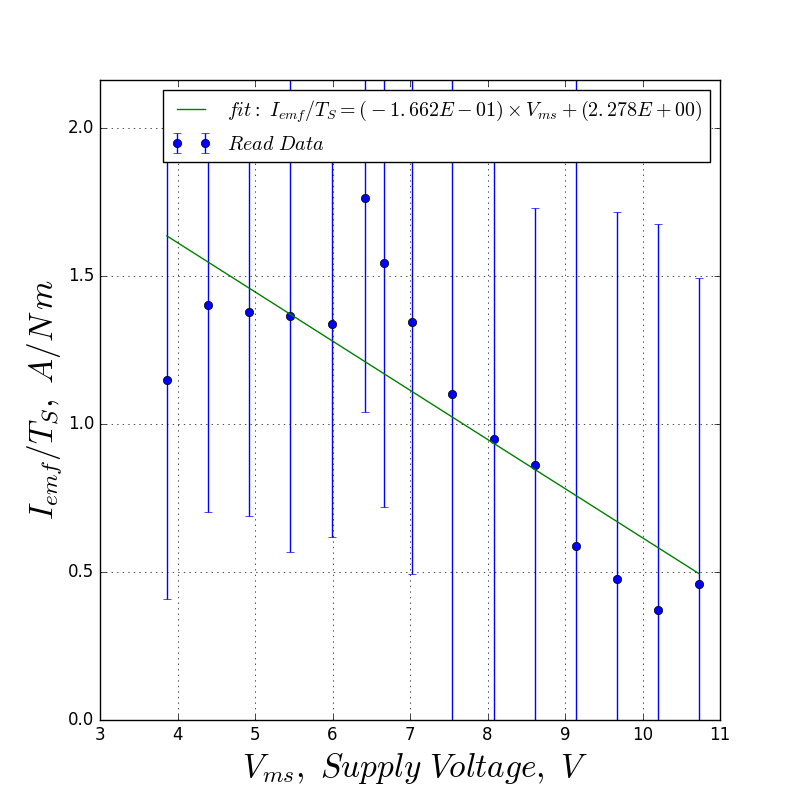
\includegraphics[scale=0.45]{figures/fig_emf_ts_cal.png}
		\caption{EMF Current \& Stall Torque Calibration Results}
		\label{figemftscal}
		\begin{subfigure}{0.9\textwidth}
			\footnotesize 
		\end{subfigure}
	\end{figure}

	\begin{equation}
		\frac{I_{emf}}{T_S} (V_{ms}) = -0.1662 \times V_{ms} + 2.278
		\label{eqnemftsend}
	\end{equation}
	
	\subsection*{Torque Calibration}
	At constant voltage, the loading on the motor was varied to produce a calibration giving the torque load on the motor as a function of the motor current supply. Each of the reference fluids (compositions on Table \ref{tabreffluvisc}) were, in turn, loaded into the motor and run at a set supply voltage. The current drawn by the motor was logged using the motor class, also used to manage the supply voltage (via the potentiometer).
	\br
	The cell was loaded with 15ml of the reference fluid. The motor was run at a supply voltage of 5.4\,V. The motor was left to run for several minutes to allow the system to come to steady state. Data from the current sensors and the dynamo was logged every millisecond. This was repeated for each of the reference fluids. With the viscosity of the reference fluids known, the torque load on the motor is therefore also known. This torque is plotted against the current drawn for each reference fluid, and a linear equation was then fit to the results, see Figure \ref{figtical}.
	\newline
	\begin{figure}[!htb]
		\centering
		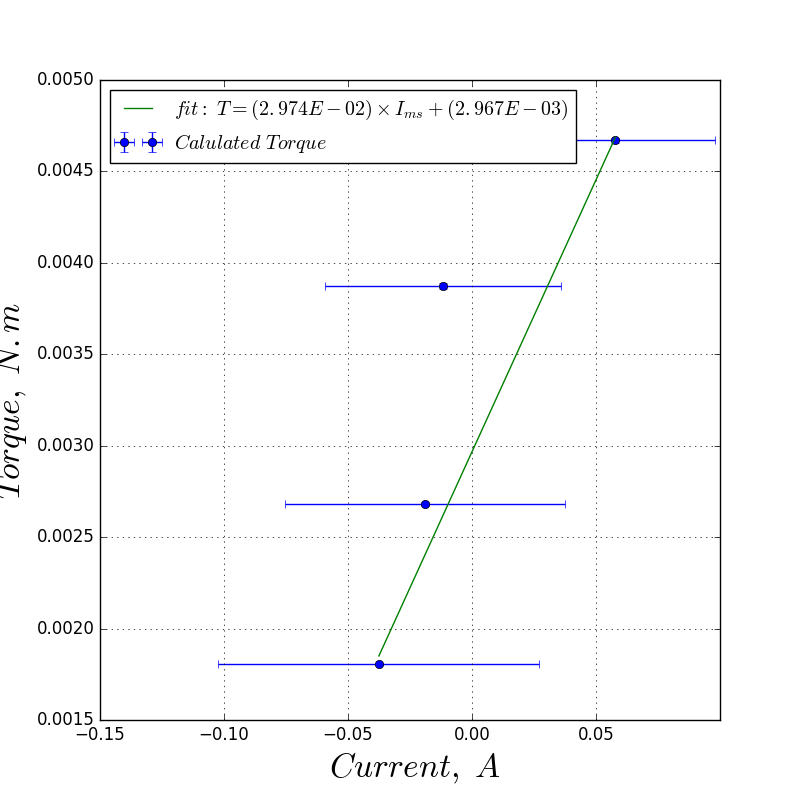
\includegraphics[scale=0.45]{figures/fig_t_ref_cal.png}
		\caption{Torque Calibration Results}
		\label{figtical}
		\begin{subfigure}{0.9\textwidth}
			\footnotesize Torque load on the motor plotted against supply current (minus free load current) at constant supply voltage (blue circles). Error bars show one standard deviation. Also plotted is a linear fit equation (green line).
		\end{subfigure}
	\end{figure}
	
	
	%=====------++++++=====------++++++=====------++++++=====------++++++=====------++++++=====------++++++=====------++++++=====------++++++=====------++++++=====------++++++=====------++++++=====------++++++
	%=====------++++++=====------++++++=====------++++++=====------++++++=====------++++++=====------++++++=====------++++++=====------++++++=====------++++++=====------++++++=====------++++++=====------++++++
	%=====------++++++=====------++++++=====------++++++=====------++++++=====------++++++=====------++++++=====------++++++=====------++++++=====------++++++=====------++++++=====------++++++=====------++++++
	%=====------++++++=====------++++++=====------++++++=====------++++++=====------++++++=====------++++++=====------++++++=====------++++++=====------++++++=====------++++++=====------++++++=====------++++++
	%=====------++++++=====------++++++=====------++++++=====------++++++=====------++++++=====------++++++=====------++++++=====------++++++=====------++++++=====------++++++=====------++++++=====------++++++
	%=====------++++++=====------++++++=====------++++++=====------++++++=====------++++++=====------++++++=====------++++++=====------++++++=====------++++++=====------++++++=====------++++++=====------++++++
	%=====------++++++=====------++++++=====------++++++=====------++++++=====------++++++=====------++++++=====------++++++=====------++++++=====------++++++=====------++++++=====------++++++=====------++++++
	%=====------++++++=====------++++++=====------++++++=====------++++++=====------++++++=====------++++++=====------++++++=====------++++++=====------++++++=====------++++++=====------++++++=====------++++++
	% Evaluation
	\nc{Evaluation}
	In this chapter, the calibrations used in the project are tested for validity, and the rheometer is evaluated against its design criteria.
	\subsection*{Voltage Control}
	To test the efficacy of the voltage control circuit, the voltage was varied (from 2.278\,V to 10.726\,V) using the digital potentiometer and measured using a voltmeter. This data was compared with the theoretical result from Equation \ref{eqnmotsupvol} and plotted in Figure \ref{figvoltvval}. This shows the read voltage supply being very close to the theoretically predicted result. A linear equation was fit to the results and compared to the theoretical, again there was excellent agreement. The circuit worked as expected.
	\begin{figure}[!htb]
		\centering
		\begin{subfigure}[t]{0.45\textwidth}
			\centering
			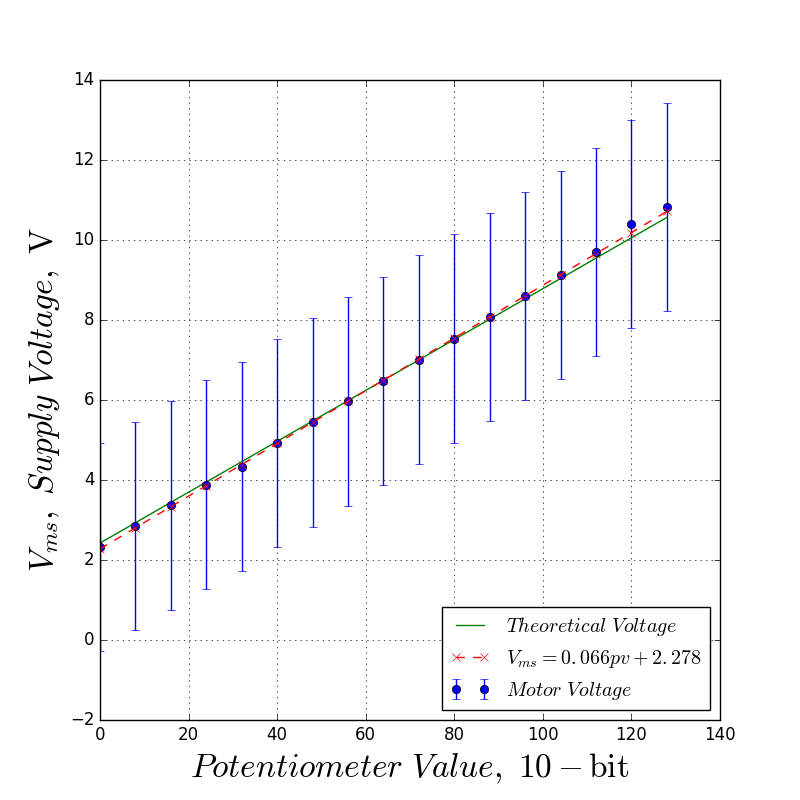
\includegraphics[scale=0.3]{figures/fig_supplyvolt_v_val.png}
			\caption{Voltage Control Check}
			\label{figvoltvval}
			\footnotesize
			Comparison of actual supply voltage (average of three readings) and theoretically expected supply voltage. A linear equation was fit to the read supply voltage data (red dashed line).
		\end{subfigure}
		\begin{subfigure}[t]{0.45\textwidth}
			\centering
			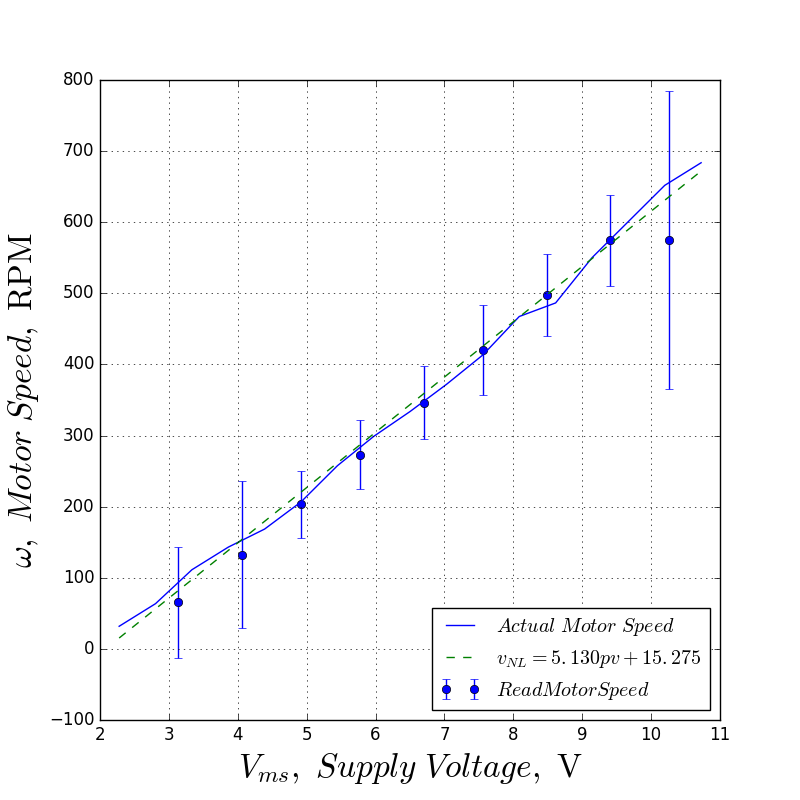
\includegraphics[scale=0.3]{figures/fig_speed_v_val.png}
			\caption{Speed Reading Check}
			\label{figdynocheck}
			\footnotesize
			Comparison of tachometer motor speed readings (blue line), and dynamo speed reading (blue circles).
		\end{subfigure}
		\label{figspeecal}
		\caption{Voltage and Speed Evaluations}
	\end{figure}
	
	\subsection*{Speed Measurement} % last edited 14/3/2017
	The rotational speed of the motor needed to be measured accurately and quickly, to be able to calculate the viscosity, and to ensure high enough sample rate that the jamming phenomenon can be seen. This was achieved by using a second motor as a dynamo, linked to the controlled motor via a belt. The dynamo will be spun and generate a voltage proportional to the rate at which it is spun, similar to the speedometer in a car. The magnitude of the voltage can be read in using an ADC by the Raspberry Pi (up to 200,000 samples per second). Accuracy of the set-up was tested using a tachometer. The recorded speeds (the tachometer results and the calibrated dynamo results) were plotted on Figure \ref{figdynocheck}. The two signals correspond fairly well, indicating that the speed measurement system works well. However, there was a fairly large amount of noise in the speed measurement signal from the dynamo. This can be seen on Figure \ref{figdynocheck} from the relatively large error bars. 
	
	\subsection*{Current Sensor}
	The sensor was calibrated by reading in from the sensor and comparing this value with the actual current reading obtained using a standard lab multimeter, repeating this at different voltages (thus also different rotational speeds and different currents). An equation was fit to the data to give an equation for the current in terms of the HES voltage. A 1$\rm ^{st}$ order equation was found to best fit the experimental results.\br
	Figures \ref{fighes30a} \& \ref{fighes5a} show how the calibrated current readings (after filtering) compare with actual values obtained using a multimeter. These values are in good agreement, although the data is somewhat noisy despite the applied filtering.
	
	\subsection*{Data Filtering}
	There were a number of options for data filtering methods to choose from. Each altered the data in different ways. The final chosen method was a Butterworth low-pass frequency filter. The other choices were a gaussian weighted average method, a Wiener filter, and using spline interpolation. Spline interpolation filters the signal by observing the shape of the response and ``drawing''a clean signal best suited. It was ruled out for not accurately following the path of the signal. The Gaussian method is a moving average, with the samples weighted according to a Gaussian normal distribution. Gaussian filtering was ruled out as it reacted to slowly to sharp changes in input readings. Wiener filtering uses statistics to estimate the desired output. The Butterworth signal was chosen as the best filter for use in the rheometer as it provided the best tracking of fluctuations in the data whilst eliminating noise.
	\br
	Figure \ref{figfiltcomp} compares the different filtering methods. A sample of noisy data (dynamo reading data) had different filters applied. The settings of each filter were altered to obtain the smoothest (noise-reduced) data without losing accuracy.
	\newline
	
	\begin{figure}[!htb]
		\centering
		\begin{subfigure}[t]{0.22\textwidth}
			\centering
			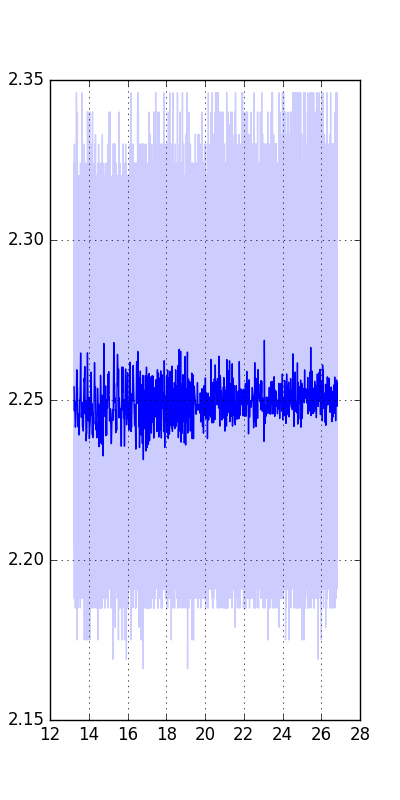
\includegraphics[scale=0.3]{figures/fig_filt_compar_spline.png}
			\caption{Spline Interpolation}
			\label{figfiltsp}
			\footnotesize
		\end{subfigure}
		\begin{subfigure}[t]{0.22\textwidth}
			\centering
			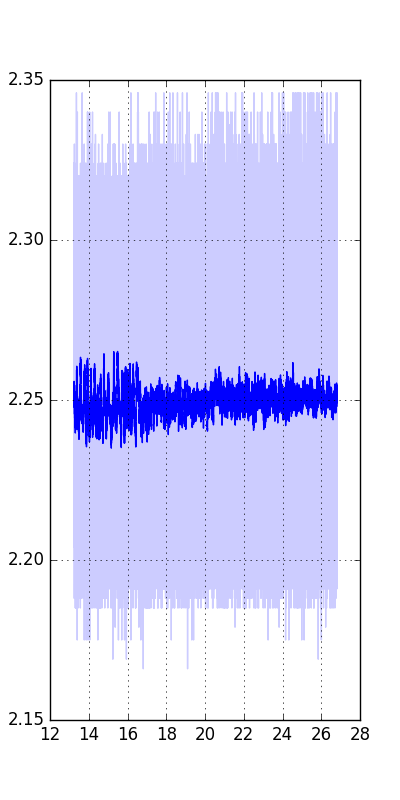
\includegraphics[scale=0.3]{figures/fig_filt_compar_wiener.png}
			\caption{Wiener Filter}
			\label{figfiltwi}
			\footnotesize
		\end{subfigure}
		\begin{subfigure}[t]{0.22\textwidth}
			\centering
			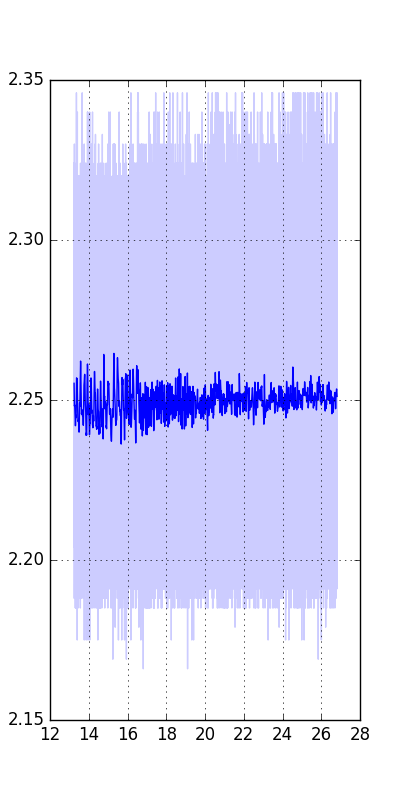
\includegraphics[scale=0.3]{figures/fig_filt_compar_gaussian.png}
			\caption{Gaussian Filter}
			\label{figfiltga}
			\footnotesize
		\end{subfigure}
		\begin{subfigure}[t]{0.22\textwidth}
			\centering
			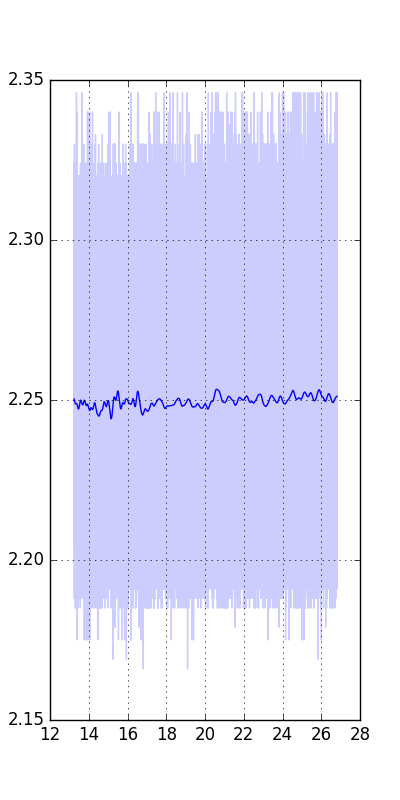
\includegraphics[scale=0.3]{figures/fig_filt_compar_butter.png}
			\caption{Butterworth Filter}
			\label{figfiltbu}
			\footnotesize
		\end{subfigure}
		\caption{Comparison of Filter Methods \label{figfiltcomp}}
	\end{figure}
	
	\noindent
	Due to the Butterworth's nature as a frequency filter, it could cause issue with reading the intermittent jumps up in viscosity due to jamming. This could be circumvented by developing a filter which recognises the different magnitude of jamming to the noise signal. Or the noise could be analysed for constituent signals: the noise could be originating from the 50Hz power supply, or another regular source. Repeated application of different band-stop filters would eliminate the known sources of noise, therefore any remaining disruption in the signal is useful data.
	\br
	In addition to Figure \ref{figfiltbu}'s example use of the Butterworth Filter, the efficacy of the algorithm can be see elsewhere. In Figure \ref{figdynocheck}, the error bars show the noise in the speed reading taken by the Dynamo. Despite the noisy signal, the filtering algorithm is able to ascertain the useful data within the signal and able to report the correct speed signal fairly accurately.
	
	\subsection*{Rheometry}
	The rheometer's ability to accurately report the viscosity of a test fluid was evaluated by using the rheometer to measure the viscosity of reference fluids of known viscosity. The results were then compared to the viscosity measurement taken using a standard lab rheometer. The rheometer was used to measure the viscosity of several reference fluids, Table \ref{tabreffluvisc} displays the compositions and viscosities of these reference fluids.
	\br
	To facilitate loading of the rheometer, the scissor lift was lowered. The outer cylinder of the rheometer was then loaded with 15\,ml of the first fluid using a 5\,ml syringe (taking care to avoid bubbles). The scissor lift was then raised into the working position; the two cylinders as close together as possible without touching. The cylinders were then aligned by turning on the motor and observing the flow of the fluid. The fluid would climb up the side of the cylinder if the inner cylinder was too close. On the Raspberry Pi a script was written which will load the motor class, with the appropriate settings, and log the data required to calculate the viscosity of the fluid in the rheometer. The motor's speed (and therefore the rate of strain experienced by the fluid) was kept constant for 5 minutes. This was repeated for each of the four reference solutions. The data was used to calculate the viscosities of the solutions as set out earlier on. The first method producing the results plotted on Figure \ref{figmures}. ed viscosities for each fluid were compared with the results obtained from the DHR-2, as plotted on Figure \ref{figrheotestres}.
	
	\nomenclature[g]{$\mu_{glycerol}$}{Viscosity of glycerol\hfill $\rm Pa\,s$}
	\nomenclature[g]{$\mu_{water}$}{Viscosity of water\hfill $\rm Pa\,s$}
	
	\noindent
	\begin{figure}[!htb]
		\centering
		\begin{subfigure}{0.45\textwidth}
			\centering
			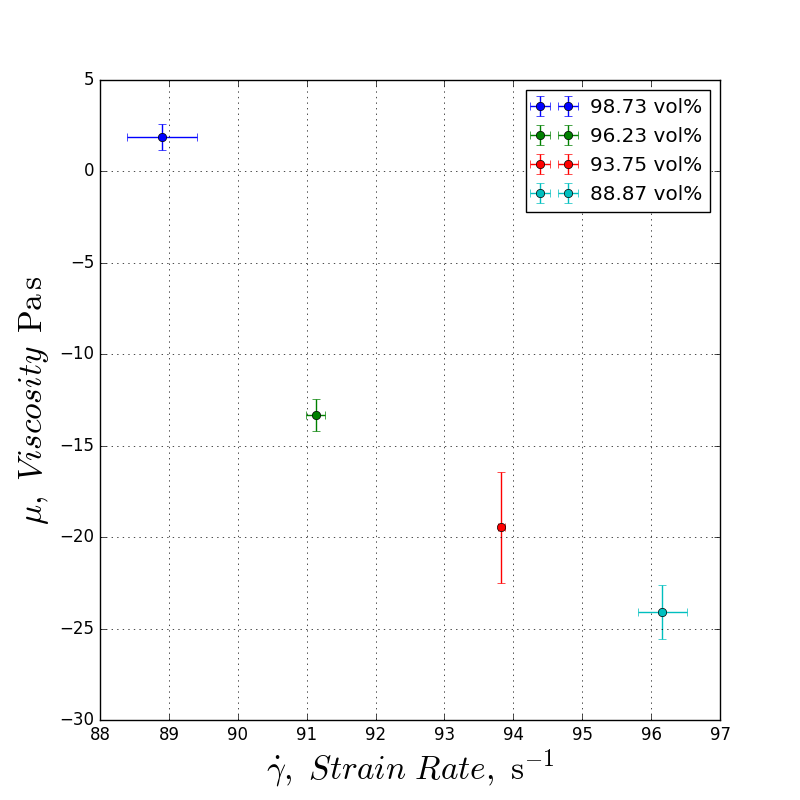
\includegraphics[scale=0.35]{figures/fig_mu_res.png}
			\caption{Method 1 Results}
			\label{figmures}
		\end{subfigure}
		\begin{subfigure}{0.45\textwidth}
			\centering
			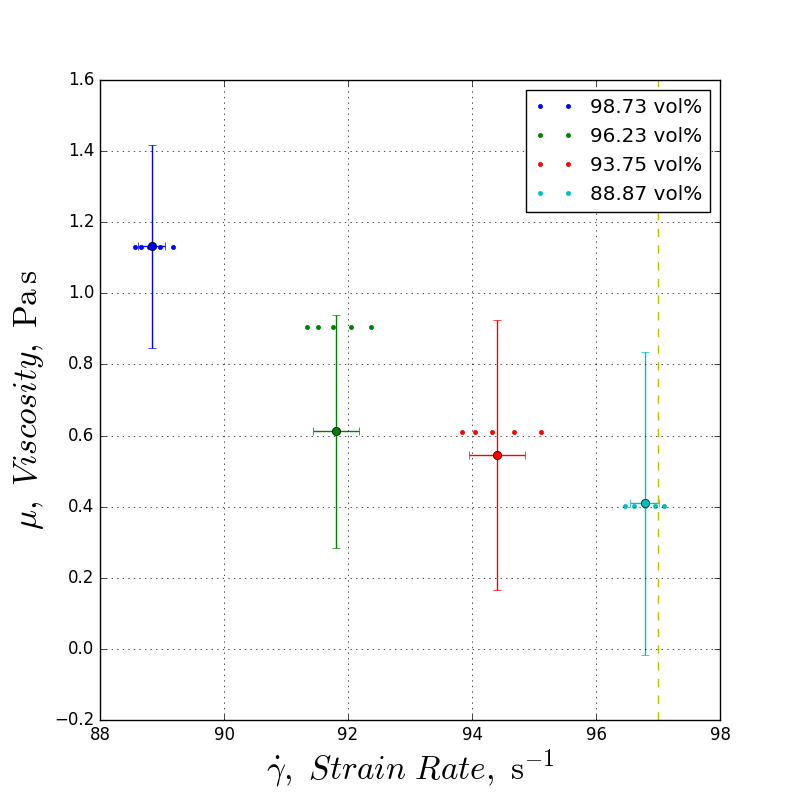
\includegraphics[scale=0.35]{figures/fig_t_ref_check.png}
			\caption{Method 2 Results}
			\label{figrheotestres}
		\end{subfigure}
		\begin{subfigure}{0.9\textwidth}
			\footnotesize Viscosity of reference fluids plotted against time. Each colour represents a different composition of reference solution (blue - 98.73v\%, green - 96.23v\%, red - 93.75v\%, and cyan - 88.87v\%). The error bars represent one standard deviation. On \textbf{(b)} the expected viscosities for each of the solutions (small circles) are also plotted as well as set strain rate for all runs (yellow dashed line).
		\end{subfigure}
	\end{figure}

	Figures \ref{figmures} \& \ref{figrheotestres} show the results of the rheometry test. The method 1 results (the results calculated by calibrating the rheometer against specific aspects of the motor's characteristic - `Calculated Method') were off the expected result by a large margin. This indicates that either the calculations and calibrations were not performed correctly, or that there was something not taken into account, or perhaps one of the assumptions made was wrong. The coil current calibration should result in a linear equation which goes directly through the origin (as it should parallel Ohm's Law). However, it was found to have an offset, indicating that that assumption is not as strong as it should be.
	\br
	Method 2's results (results from a straight calibration of the motor's torque to the supply current at constant voltage - `Calibrated Method') agree better with the expected results (3 out of 4 runs gave an average viscosity in good agreement to the expected viscosity). The second result could be an outlier for several reasons: it could have been slightly warmer than expected (temperature was not recorded), or water could have contaminated the sample. However, the latter is unlikely: the samples were sealed shortly after they were produced and not opened again until tested. This method provides good results, however it can only be used at constant voltage - therefore there would be no control over either the strain rate or the 
	
	\subsection*{Control}
	The control system was tested by writing a script to read in the motor's speed, which was converted into a control action using the control class which was applied to the digital potentiometer. This was repeated every 100\,ms for 5 minutes. The motor class was used in the script to read the motor's speed, and to set the new supply voltage. The script was extended to log information (potentiometer value, speed, current, control action) about the process' response to a change in set point and amongst disturbances.
	\br
	Before the controller could be used, it needed to be tuned. The tuning was obtained by first introducing a step change in the supply voltage to gauge how the speed (controller input) is affected by the potentiometer value (controller output). A First Order Plus Dead Time (FOPDT) transfer function model was used to model the controller's response under different tunings, the optimal tuning settings found simply by trial and error.
	\br
	Trial and error tuning is simple, but is time consuming. The control class's tune function was used along with trial and error fine tuning to obtain the optimal tuning parameters for the controller. The testing script was then run with the optimal tuning.
	\newline
	
	\begin{figure}[!htb]
		\centering
		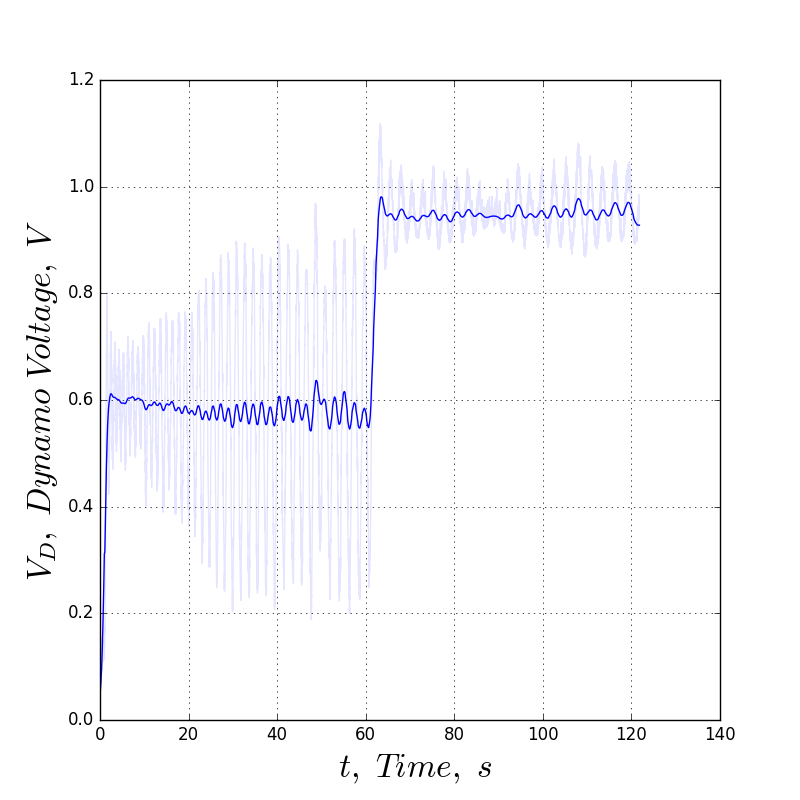
\includegraphics[scale=0.45]{figures/fig_contr_test.png}
		\caption{Controller Test}
		\label{figcontrtest}
		\begin{subfigure}{0.6\textwidth}
			\footnotesize Raw dynamo reading data plotted against time (faint blue line). Filtered dynamo readings plotted against time (bright blue line). The oscillation in the response can be seen clearly.
		\end{subfigure}
	\end{figure}
	
	\noindent
	Figure \ref{figcontrtest} shows the ineffectiveness of the control system. The response oscillates around the set point. This could be an issue with the tuning (gains set too high). This could also be an issue with resolution; the digital potentiometer can only give 128 different combinations (therefore 128 possible different supply voltages). In addition, the live filter applied to the data used by the control system creates dead time of around 100\,ms (100 samples of lag for the motor speed measurement process, but only 1 sample as far as the control system is concerend). This means that the control system doesn't react to outside stimuli as fast as it could; this is maybe why it oscillates. A Smith predictor (used to compensate for lag, also known as dead-time), but the model of the process would have to be improved for this to be a viable option \cite{smithref}.
	\br
	There is a clear need for the control system. Looking at Figure \ref{figrheotestres}, it can be seen that the different fluids are sheared at different rates due to their different viscosities. If the viscosity is not known (as would be expected for a fluid placed into a rheometer) this drift from the zero viscosity strain rate cannot be predicted. Instead, a control system should be in place to monitor the speed of the motor and maintain it at a set point to ensure that a desired strain rate is maintained.
	
	\subsection*{Design Criteria}
	The design criteria laid out at the beginning were that the rheometer should:
	\begin{itemize}
		\item be able to calculate the viscosity of a fluid as it varies with time.
		\item be operationally modular (easy to alter the exact parameters with which it runs).
		\item be low-cost (under \pounds 100).
	\end{itemize}
	The final design consisted of a Raspberry Pi (\pounds 30), some electronic hardware (ADC -- \pounds 3, HECS sensors -- \pounds 5 $\times$ 3, resistors -- \pounds nil, operational amplifiers -- \pounds 7, breadboard -- \pounds 10, and wires -- \pounds nil), a DC motor (\pounds 5), Two cylinders (estimated \pounds 11) and various pieces of lab equipment (clamp stand, scissor lift etc.). All of this together (around \pounds 70) is below the target of \pounds 100 and well below the cost of a satndard laboratory rheometer (on the order of tens of thousands of pounds). In this regard, the rheometer has met its target.
	The device is controlled entirely via scripts using the python classes developed over the course of this project, resulting in a system which can be tweaked and altered depending on the needs of the situation. Again, in this regard the rheometer has met its target.
	Finally, the rheometer did not quite meet its target for viscosity measurement: it is able to do so selectively and without speed control, but this is not enough to meet the objectives set out. For the rheometer to work fully, it needs to be able to be speed controlled (thus setting the strain rate). A more complete version of the torque calibration would enable the calculation to be done at any supply voltage -- allowing the speed to be controlled and therefore constant strain rate operation to be undertaken.
	
	%=====------++++++=====------++++++=====------++++++=====------++++++=====------++++++=====------++++++=====------++++++=====------++++++=====------++++++=====------++++++=====------++++++=====------++++++
	% Conclusion and Discussion
	\nc{Conclusions and Discussion}
	The rheometer works, but only for giving mean values of viscosity and when calibrated at a specific supply voltage. This is not enough for it to meet the brief, and there is work yet to be done for it to meet all of the objectives. The first method of calculating the viscosity is a very promising model, but is not complete as yet. This is one area that could be used to improve the results. In addition, quantitative speed and current sensors could be used to get a direct idea of the current supply to the motor and its speed. This would also eliminate the possibility of sensor drift - the sensor giving different readings over time and therefore the calibrations no longer being valid. Also, a temperature sensor should be added to monitor the temperature the system is measuring viscosity at. Temperature has a not-insignificant effect on the viscosity of several fluids (glycerol has a viscosity of around 3\,Pa\,s at 10$\rm^oC$) and 1.4\,Pa\,s at 20$\rm^oC$) and therefore it would be useful to record this information. 
	\br
	% FUTURE WORK
	Future work could include: changing out the motor for a motor torque-sensitive model, introducing a piezo-electric stress sensor, and adding a camera for detecting optical evidence of jamming. Piezo electrics are often used as strain sensors in bridges and other systems. Previous work has used the strain sensor as a purely qualitative way of examining jamming (\cite{thescforsyth}). By relating the force observed on the piezo sensor to the drag coefficient of the sensor in the flowing fluid, and therefore the fluid's Reynold's number, the viscosity can be related to the voltage output of the piezo electric device. 
	\br
	Another future step to take with the project would be to use the control system developed along with the addition of some current control circuit to be able to control the shear stress (by controlling the motor torque). This would increase the utility of the rheometer by adding a second operational mode with controlled/constant shear stress as opposed to constant shear rate as it is at the moment.
	\br
	Complementary to the temperature sensor mentioned previous, some temperature control system would be extremely useful for the rheometer. Temperature control is normally included in other lab-based rheometers, usually in the form of a water jacket.
	
%% APPENDIX %%
	%=====------++++++=====------++++++=====------++++++=====------++++++=====------++++++=====------++++++=====------++++++=====------++++++=====------++++++=====------++++++=====------++++++=====------++++++
	% Reflection and Review
	
	\nc{Reflection and Review}
	Over the course of the project I have learned a lot. I have had to learn new things; I have had to improve pre-existing skills. The python language (and \LaTeX) was completely new to me at the start of the project. Although I have previous programming experience; I had to very quickly become familiar with new concepts and ways of thinking. The software development process was very segmented - some parts could be written and tested very quickly, others had to be tested with the rheometer hardware. Also, with hardware changes, the software had to be altered to suit. Sometimes, this meant loss of hours of work due to the code no longer being required. But this time was not lost. For example, I spent a day examining the datasheet for an ADC and pouring over the specification sheets for the $\rm I^2C$ serial communication protocol. However, I couldn't solder the ADC onto the breakout-board (I lacked both the skills and equipment). Rather than sinking more time into fine-tuning my soldering skills, a new ADC was found (which did not require soldering but had a lower resolution). This ADC used the SPI protocol and so didn't need the $\rm I^2C$ code I had written previously. However, with my experience of working with serial data transfer and reading datasheets, the new SPI code didn't take any time at all to write.
	\br
	Working with the Raspberry Pi has taught me a lot about how computers work, how they communicate, and how they may be used in industrial processes. Data processing and storage has been an important concern; with the Raspberry Pi taking thousands of measurements every second. The Pi only has limited memory available, which can fill up quickly. This was circumvented by saving the data to file, rather than keeping it in memory. 
	\br
	Another area I gained a lot of experience with was data processing. Data recorded from sensors was noisy - due to random fluctuations in temperature, air pressure, vibrations, power supply. The noise was reduced using a filtering algorithm. As I was researching noise filtering I learned about the types of filters and how they work, I learned about how different signal domains (like the frequency domain) can be used to remove unwanted parts of the signal.
	\br
	The project has had me trying new ideas and testing them to see if they work; if they don't I had to move on, to try something else. A good example of this is the speed sensor. Originally I was going to use a hall effect sensor to sense the presence of a magnet - this could be recorded by the Raspberry Pi and used to calculate the speed. However (despite my many attempts and alterations) this method did not work. I moved on, tried a similar method using a light gate. This method resulted in similar disappointment so I moved on to a fully different method - the dynamo. This method is not as accurate as the other methods tried would have been, but it is reliable. This is typical of many things I tried in the report. I have definitely learned determination through this project; it would have been easy to lose focus after the first or second mishap, but I learned to keep going and move on and try another idea.
	\br
	Twelve weeks may seem like a long time, but it was actually very tight. The development process ran long, resulting in things not being finished, some were not even started. Over the course of the project, I certainly became practised in prioritising some areas of the work over others; The speed sensor was extremely troublesome and time consuming -- but is essential to the project so the time was not wasted. The control system I could not get working perfectly -- but I could not sink too much time into as it was not strictly necessary to obtain a viscosity reading from the rheometer.
	
	%=====------++++++=====------++++++=====------++++++=====------++++++=====------++++++=====------++++++=====------++++++=====------++++++=====------++++++=====------++++++=====------++++++=====------++++++
	% Nomenclature
	\newpage
	\stepcounter{chapter}
	\addcontentsline{toc}{chapter}{Nomenclature}
	\def\achapter{Nomenclature}
	%List all the symbols in alphabetical order, with Greek symbols at the end
	\printnomenclature[1.5cm]
	
	%=====------++++++=====------++++++=====------++++++=====------++++++=====------++++++=====------++++++=====------++++++=====------++++++=====------++++++=====------++++++=====------++++++=====------++++++
	% Main Bibliography
	\newpage
	\addcontentsline{toc}{chapter}{Bibliography}
	\def\achapter{Bibliography}
	%\bibliographystyle{unsrt}
	\bibliographystyle{apalike}
	\bibliography{biblio}




\appendix


\chapter*{Appendices}
%appendix preamble

\addcontentsline{toc}{chapter}{Appendices}
\def\achapter{Appendices}
\pagenumbering{alph}
\setcounter{page}{1}
\setcounter{secnumdepth}{0}
\setcounter{section}{1}

\newcounter{apsec}
\setcounter{apsec}{0}
\newcounter{apsubsec}
\def\apsect#1{
	\addtocounter{apsec}{1}
	\section{\arabic{apsec}\hskip0.5cm #1}
	\setcounter{apsubsec}{1}
}
\def\apsubsect#1{
	\subsection*{\arabic{apsec}\Alph{apsubsec} \hskip0.5cm #1}
	\addtocounter{apsubsec}{1}
}

\apsect{Source Code}
%-=-=-=-=-=-=-=-=-=-=-=-=-=-=-=-=-=-=-=-=-=-=-=-=-=-=-=-=-=-=-=-=-=-=-=-=-=-=-=-=-=-=-=-=-=-=-=-=-=-=-=-=-=-=-=-=-=-=-=-=-=--=-=-=-=-=-=-=-=-=-=-=-=-=-=-=-=-=-=-=-=-=-=-=-=-=-=-=-=-=-=-=-=-=-=-=-=-=-=-=-=-=-=-=-=-=-=-=-=-=-=-=-=-=-=-=-=-=-=-=-=-=-=-=-=-=-=-=-=-=-=-=-=
As mentioned previously, the software was split up into different sections. This was to make the code more manageable, and easier to maintain. The source code for each class section, as well as the filtering library, is included here:
\renewcommand{\labelenumi}{\Alph{enumi}}
\begin{enumerate}
	\item -- ``adc.py'' -- ADC class source code
	\item -- ``dig\_pot.py'' -- digital potentiometer class source code
	\item -- ``motor.py'' -- motor class source code
	\item -- ``control.py'' -- controller class source code
	\item -- ``filter.py'' -- filter library source code
\end{enumerate}
\apsubsect{ADC Class}
%-=-=-=-=-=-=-=-=-=-=-=-=-=-=-=-=-=-=-=-=-=-=-=-=-=-=-=-=-=-=-=-=-=-=-=-=-=-=-=-=-=-=-=-=-=-=-=-=-=-=-=-=-=-=-=-=-=-=-=-=-=--=-=-=-=-=-=-=-=-=-=-=-=-=-=-=-=-=-=-=-=-=-=-=-=-=-=-=-=-=-=-=-=-=-=-=-=-=-=-=-=-=-=-=-=-=-=-=-=-=-=-=-=-=-=-=-=-=-=-=-=-=-=-=-=-=-=-=-=-=-=-=-=

\begin{Verbatim}[frame=single,fontsize=\footnotesize]
import RPi.GPIO as gpio
import spidev as spi


class MCP3008(object):
	
	bus = 0  # holds the bus connection
	cs_pin = 0  # which GPIO pin is used to talk to this chip? (gpio.BOARD numbering) 
				# OR which cs channel to use
	vref = 3.3  # Reference voltage in use
	
	def __init__(self, cs_pin=1, vref=3.3):
		''' 
		object = adc.MCP3008(**kwargs)
		
		Initialise MCP3008 ADC class object.
		
		kwargs:
		cs_pin - SPI chip select. Default is 1.
		vref - ADC reference voltage. Default is 3.3.
		'''
		
		# Chip select setup
		self.cs_pin = cs_pin
		if (cs_pin > 1):  
			# using the GPIO pins as chip_select pins
			gpio.setmode(gpio.BOARD)
			
			# chip select is normally high, 
			# pulled up by the RPi, 
			# just like many GPIO, 
			# its not electrically low
			gpio.setup(self.cs_pin, gpio.OUT, pull_up_down=gpio.PUD_UP)
			
			gpio.output(self.cs_pin, gpio.HIGH)
		else:  
			# using the Pi's built in chip select method
			pass
		
		# Set up bus connection
		self.bus = spi.SpiDev()
		
		# Vref setting
		self.vref = vref
	
	def read_data(self, channel):
		'''
		read_data(channel)
		
		Converts the voltage (relative to vref) on the specified channel to a 
		10-bit number.
		
		channel - (int, 0-7) the ADC data channel that is to be read from.
		
		returns: (int, 0-1023) 10-bit value indicating the voltage on 
		          the channel specified.
		'''
		
		self.open()
		indat = self.bus.xfer2([1, 8 + channel << 4, 0])
		self.close()
		return ((indat[1] & 3) << 8) + indat[2]
	
	def read_volts(self, channel):
		'''
		read_volts(channel)
		
		Reads the voltage level on the specified channel.
		
		channel - (int, 0-7) the ADC data channel that is to be read from.
		
		returns float representing the voltage level on the channel specified.
		'''
		
		dat = self.read_data(channel)
		volts = (float(dat) / 1024.0) * self.vref
		return volts
	
	def write_byte(self, byte):
		'''
		write_byte(byte)
		
		byte - the 8 bit command to be sent to the ADC.
		'''
		
		self.open()
		command = [byte, 0]  # Two bytes:
		                     # first is command shifted 4 bits, 
		                     # second is zero
		self.bus.writebytes(command)
		self.close()
	
	def open(self):
		'''
		open()
		
		opens a channel to the SPI device.
		
		Must completed by a following close() call.
		'''
		if (self.cs_pin > 1):
			gpio.output(self.cs_pin, gpio.HIGH)
			self.bus.open(0, 1)
			self.bus.max_speed_hz = 10000000
		else:
			self.bus.open(0, self.cs_pin)
			self.bus.max_speed_hz = 10000000
	
	def close(self):
		'''
		close()
		
		closes a (previously opened) channel to the SPI device.
		'''
		if (self.cs_pin > 1):
			gpio.output(self.cs_pin, gpio.LOW)
			self.bus.close()
		else:
			self.bus.close()
\end{Verbatim}
\apsubsect{Digital Potentiometer Class}
%-=-=-=-=-=-=-=-=-=-=-=-=-=-=-=-=-=-=-=-=-=-=-=-=-=-=-=-=-=-=-=-=-=-=-=-=-=-=-=-=-=-=-=-=-=-=-=-=-=-=-=-=-=-=-=-=-=-=-=-=-=--=-=-=-=-=-=-=-=-=-=-=-=-=-=-=-=-=-=-=-=-=-=-=-=-=-=-=-=-=-=-=-=-=-=-=-=-=-=-=-=-=-=-=-=-=-=-=-=-=-=-=-=-=-=-=-=-=-=-=-=-=-=-=-=-=-=-=-=-=-=-=-=
\begin{Verbatim}[frame=single,fontsize=\footnotesize]
import spidev as spi

class MCP4131(object):
	'''
	SPI 10K Digital Potentiometer
	'''
	bus = 0  # holds the bus connection to the digital pot
	lav = 0
	chip_select = 0
	
	def __init__(self, chipselect=0):
		'''
		MCP4131()
		
		Creates an instance of the MCP4131 class for communicating over SPI with
		an MCP4131 digital potentiometer.
		
		kwargs:
		chipselect -  the chip_select address for the MCP4131 chip on the 
		              SPI network.
		'''
		self.bus = spi.SpiDev()
		self.chip_select = chipselect
	
	def set_resistance(self, value):
		'''
		set_resistance(value)
		Sets the value on the potentiometer.
		
		value - integer value to set on the potentiometer. The resistance betweeen 
		        the A terminal and the wiper will vary directly with this value.
		'''
		self.lav = value
		self.write_byte(value)
	
	def write_byte(self, byte):
		'''
		write_byte(byte)
		
		Writes the specified byte to the digital potentiometer.
		
		byte - the value to send to the potentiometer.
		'''
		self.open()
		command = [0, byte]
		self.bus.writebytes(command)
		self.close()
	
	def open(self):
		'''
		open()
		
		Begins communication with the potentiometer.
		Must be matched by an accompanying "close()"
		'''
		self.bus.open(0, self.chip_select)
		self.bus.max_speed_hz = 10000000
	
	def close(self):
		'''
		close()
		
		Ends communication with the potentiometer.
		'''
		self.bus.close()
\end{Verbatim}
\apsubsect{Motor Class}
%-=-=-=-=-=-=-=-=-=-=-=-=-=-=-=-=-=-=-=-=-=-=-=-=-=-=-=-=-=-=-=-=-=-=-=-=-=-=-=-=-=-=-=-=-=-=-=-=-=-=-=-=-=-=-=-=-=-=-=-=-=--=-=-=-=-=-=-=-=-=-=-=-=-=-=-=-=-=-=-=-=-=-=-=-=-=-=-=-=-=-=-=-=-=-=-=-=-=-=-=-=-=-=-=-=-=-=-=-=-=-=-=-=-=-=-=-=-=-=-=-=-=-=-=-=-=-=-=-=-=-=-=-=
\begin{Verbatim}[frame=single,fontsize=\footnotesize]
import time
import os
import thread as td
import RPi.GPIO as gpio
import filter
from glob import glob
from dig_pot import MCP4131 as dp
from adc import MCP3008 as ac
from control import tf_pi_controller as pitf


class motor(object):

	# Internal Switches
	poll_running = False  # is the speed currently being polled?
	
	# Logging
	poll_logging = True  # Will log every (i_poll_rate)s if this is True
	log_paused = False
	log_add_note = False
	log_dir = "./logs"  # where the logged data should be saved
	i_poll_rate = 0.1  # How often data is polled, should not be less than span
	this_log_name = ""
	
	# Speed calc
	speed = 0.0  # Output value
	dr = 0.0
	fdr = 0.0
	svf = [300, -150]  # 1st order linear fit equation; 
	                   # SPEED = svf[0] * VOLTAGE + svf[1];
	                   # VOLTAGE in volts, SPEED in RPM
	
	# Filtering
	filtlen = 1000    # number of samples to "remember" for filtering purposes
	srvs = [0.0] * 0  # used to hold the last (filtlen) samples of dynamo volt readings
	crvs = [0.0] * 0  # used to hold the last (filtlen) samples of current volt readings
	tims = [0.0] * 0  # time data for ^
	filtering = "NONE"
	filter_delay = 100
	filtA = 2
	filtB = 0.008
	
	# Control thread
	control_stopped = True
	
	# Sub-classes
	pot = dp()  # potentiometer to control voltage
	pic = pitf((0.2, 0.15))
	aconv = ac()  # adc to read current/voltage
	adc_chan = [0, 1, 2, 3]  # voltage channel, HES30A, HES5A x2
	
	def __init__(self, startnow=False, adc_channels=[0, 1], adc_vref=3.3,
	             poll_logging=True, log_dir="./logs",
	             log_name="DATETIME", svf=[312.806, -159.196], i_poll_rate=0.1, 
	             pic_tuning=(0.2, 0.15), filtering="NONE", filter_samples=100, 
	             filt_param_A=0.314, filt_param_B=0.314):
		
		# Set calibration variables
		self.svf = svf
		
		# controller
		self.pic = pitf(pic_tuning)
		
		# Filtering
		self.filtering = filtering
		if not filtering == "NONE": self.filtlen = filter_samples
		if not filt_param_A == 0.314: self.filtA = filt_param_A
		if not filt_param_B == 0.314: self.filtB = filt_param_B
		
		# Set sensor variables
		#self.pot = dp()
		#self.aconv = ac(cs_pin=1, vref=adc_vref)
		self.i_poll_rate=i_poll_rate
		
		# Set up logs
		self.log_dir = log_dir
		self.poll_logging = poll_logging
		self.new_logs(log_name)
		
		# Start speed polling (if necessary)
		if (startnow):
			self.start_poll()
	
	def new_logs(self, log_name="DATETIME"):
		# Try closing old log file
		try:
			logf.close()
		except:
			pass
		
		# Check if log directory exists. If not, create it.
		if not os.path.isdir(self.log_dir):
			os.mkdir(self.log_dir)
		
		# Get unique number for the log file
		un = time.strftime("%H %M %S", time.gmtime())
		
		# Creat log
		if (self.poll_logging):
			if log_name == "DATETIME":
				self.this_log_name = self.log_dir + "/log_" + un + ".csv"
			else:
				self.this_log_name = self.log_dir + "/" + log_name
			
				self.logf = open(self.this_log_name, "w")
			
				self.logf.write("t,dr,cr,cr2a,cr2b,pv,fdr,fcr\n")
	
	def log_pause(self):
		self.log_paused = True
	
	def log_resume(self, new_note="resumed"):
		self.log_note = new_note
		self.log_paused = False
	
	def start_poll(self):
		if (not self.poll_running):  # if not already running
			td.start_new_thread(self.poll, tuple())
	
	def start_control(self):
		if self.control_stopped:
			self.control_stopped = False
			td.start_new_thread(self.control, tuple())
	
	def update_setpoint(self, value):
		self.pic.set_point = value
	
	def control(self):
		while not self.control_stopped:
			control_action = self.pic.get_control_action(self.speed)
			if control_action > 128: control_action = 128
			if control_action < 0: control_action = 0
			self.set_pot(control_action)
			time.sleep(0.1)
	
	def stop_control(self):
		self.control_stopped = True
	
	def poll(self):
	
		self.poll_running = True
		
		while (self.poll_running):
		
			t = time.time()
			
			# Get speed and current sensor readings
			volts = [self.aconv.read_volts(self.adc_chan[0]), 
			         self.aconv.read_volts(self.adc_chan[1]), 
			         self.aconv.read_volts(self.adc_chan[2]), 
			         self.aconv.read_volts(self.adc_chan[3])]
			self.dr = volts[0]
			fvolts = volts
			
			# if desired, apply filtering to input
			if not (self.filtering == "NONE"):
				self.update_filt_hist(volts[0], volts[1], t)
				start_delay = 20
			
			if (len(self.tims) >= start_delay):
				fvolts[0] = filter.filter(self.tims, 
				                          self.srvs, 
				                          method=self.filtering, 
				                          A=self.filtA, 
				                          B=self.filtB)[-10]
				fvolts[1] = filter.filter(self.tims, 
				                          self.crvs, 
				                          method=self.filtering, 
				                          A=self.filtA, 
				                          B=self.filtB)[-10]
			
			self.fdr = fvolts[0]
			self.speed = self.fdr * self.svf[0] + self.svf[1]
			
			if self.log_paused:
				self.log_add_note = True
			
			if (self.poll_logging) and (not self.log_paused):
				if self.log_add_note:
					self.logf.write(("{0:.6f}, {1:.3f}, {2:.3f}, 
					               {7:.3f}, {8:.3f}, {3}, 
					               {4:.3f}, {5:.3f}, {6} 
					               \n").format(
					               t, volts[0], volts[1], 
					               self.pot.lav, fvolts[0], fvolts[1], 
					               self.log_note, volts[2], volts[3]))
					self.log_add_note = False
				else:
					self.logf.write(("{0:.6f}, {1:.3f}, {2:.3f}, 
					               {6:.3f}, {7:.3f}, {3}, 
					               {4:.3f}, {5:.3f} 
					               \n").format(
					               t, volts[0], volts[1], 
					               self.pot.lav, fvolts[0], fvolts[1], 
					               volts[2], volts[3]))
			
			# delay for x seconds
			time.sleep(self.i_poll_rate)
		
		print("Motor polling has halted.")
	
	def update_filt_hist(self, srv, crv, tim):
		if (len(self.srvs) + 1) > self.filtlen:
			self.srvs = self.srvs[1:]
			self.crvs = self.crvs[1:]
			self.tims = self.tims[1:]
		self.srvs.append(srv)
		self.crvs.append(crv)
		self.tims.append(tim)
	
	def set_pot(self, value):
		self.pot.set_resistance(int(value))
	
	def clean_exit(self):
		self.poll_running = False
		self.control_stopped = True
		time.sleep(0.5)
		
		if (self.poll_logging):
			self.logf.close()
\end{Verbatim}
\apsubsect{Controller class}
%-=-=-=-=-=-=-=-=-=-=-=-=-=-=-=-=-=-=-=-=-=-=-=-=-=-=-=-=-=-=-=-=-=-=-=-=-=-=-=-=-=-=-=-=-=-=-=-=-=-=-=-=-=-=-=-=-=-=-=-=-=--=-=-=-=-=-=-=-=-=-=-=-=-=-=-=-=-=-=-=-=-=-=-=-=-=-=-=-=-=-=-=-=-=-=-=-=-=-=-=-=-=-=-=-=-=-=-=-=-=-=-=-=-=-=-=-=-=-=-=-=-=-=-=-=-=-=-=-=-=-=-=-=
\begin{Verbatim}[frame=single,fontsize=\footnotesize]
from time import time
from time import sleep
import sys
import matplotlib.pyplot as plt
import scipy.signal as sg
import numpy as np
import warnings

class tf_pi_controller(object):
	'''
	object = tf_pi_controller(tuning, set_point)
	
	Creates an instance of a PI controller.
	
	args:
	tuning      -   tuple: (float, float). Represents the gain parameters Kc and 
	                Kc/Ti respectively
	                
	set_point   -   float. Represents the desired output from the process. 
	                Default is 0
	                
	sample_time -   float. Time between iterations in seconds. 
	                Default is 0.1
	
	accessible data:
	tuning      -   tuple: (float, float). Represents the gain parameters 
	                Kc and Kc/Ti respectively
	                
	set_point   -   float. Represents the desired output from the process. 
	                Default is 0
	
	Ys          -   list, float. List of past process outputs.
	Us          -   list, float. List of past controller outputs.
	Es          -   list, float. List of past error values.
	
	remd_len    -   integer. "Remembered Length" number of items to remember. 
	                Default is 100.
	'''
	tuning = [0.0, 0.0]
	
	set_point = 0.0
	
	Ys = [0.0] * 2
	Us = [0.0] * 2
	Es = [0.0] * 2
	
	remd_len = 100
	
	def __init__(self, tuning, set_point=0.0, sample_time=0.1):
		'''
		object = tf_pi_controller(tuning, set_point)
		
		Creates an instance of a PI controller.
		
		args:
		tuning      -   tuple: (float, float). Represents the gain parameters 
		                Kc and Kc/Ti respectively
		                
		set_point   -   float. Represents the desired output from the process. 
		                Default is 0
		                
		sample_time -   float. Time between iterations in seconds. 
		                Default is 0.1
		'''
		self.tuning = tuning  # Set tuning
		self.set_point = set_point  # Set set point
		with warnings.catch_warnings():
			warnings.simplefilter("ignore")
			# create controller transfer function
			self.Gc = sg.TransferFunction((self.tuning[0], 
			                               self.tuning[1]), 
			                               (1, 0), 
			                               dt=sample_time)
	
	def get_control_action(self, Y):
		# set next input and error values in memory
		self.Ys.append(Y)
		self.Es.append(self.set_point - Y)
	
		# Tidy up memory
		if len(self.Ys) > 100: Ys = self.Ys[1:]
		if len(self.Es) > 100: Ys = self.Es[1:]
		
		# apply controller transfer function
		self.Us = self.Gc.output(self.Es, range(0, len(Es)))[1]
		
		return self.Us[-1]
	
	def do_sim(self, time_constant, steady_state_gain, sp=0, 
	           step_to=200, at_t=10, length=100):
		'''
		do_sim(time_constant, steady_state_gain, sp_step=200, at_t=10, length=100)
		
		Simulates the controller's response to a step change in set point.
		
		args:
		time_constant - float. Coefficient of s in denominator of transfer function
		steady_state_gain - float. Numerator of transfer function.
		
		kwargs**:
		sp          -   float. Initial set point. 
		                Default is 0.0
		                
		step_to     -   float. Final set point. 
		                Default is 200.0
		                
		at_t        -   integer. Number of samples to wait before stepping up. 
		                Default is 10
		                
		length      -   integer. Number of samples overall to compute. 
		                Default is 100
		'''
		set_point = sp
		# Set up transfer functions
		Gp = sg.TransferFunction((steady_state_gain), (time_constant, 1))
		Gc = sg.TransferFunction((self.tuning[0], self.tuning[1]), (1, 0))
		
		# Create initial conditions
		Ys = [0, 0]
		Es = [0, 0]
		Us = [0, 0]
		
		for i in range(0, at_t):
		# Apply process transfer function to inputs
		Ys.append(Gp.output(Us, range(0, len(Us)))[1][-1])
		
		# Get new error
		Es.append(set_point - Ys[-1])
		
		# Apply controller transfer function to inputs
		Us = Gc.output(Es, range(0, len(Es)))[1]
		
		set_point = step_to
		
		for i in range(0, length - at_t):
		# Apply process transfer function to inputs
		Ys.append(Gp.output(Us, range(0, len(Us)))[1][-1])
		
		# Get new error
		Es.append(set_point - Ys[-1])
		
		# Apply controller transfer function to inputs
		Us = Gc.output(Es, range(0, len(Es)))[1]
		
		Ts = np.array(range(0, len(Ys))) * 0.1 - 0.2
		return (Ys, Es, Us, Ts)
\end{Verbatim}
\apsubsect{Filtering}
%-=-=-=-=-=-=-=-=-=-=-=-=-=-=-=-=-=-=-=-=-=-=-=-=-=-=-=-=-=-=-=-=-=-=-=-=-=-=-=-=-=-=-=-=-=-=-=-=-=-=-=-=-=-=-=-=-=-=-=-=-=--=-=-=-=-=-=-=-=-=-=-=-=-=-=-=-=-=-=-=-=-=-=-=-=-=-=-=-=-=-=-=-=-=-=-=-=-=-=-=-=-=-=-=-=-=-=-=-=-=-=-=-=-=-=-=-=-=-=-=-=-=-=-=-=-=-=-=-=-=-=-=-=
\begin{Verbatim}[frame=single,fontsize=\footnotesize]
import numpy as np
from scipy.interpolate import UnivariateSpline
from scipy.signal import wiener, filtfilt, butter, gaussian
from scipy.ndimage import filters

def gaussianf(x, y, sample_size=51, sigma=7):
	b = gaussian(sample_size, sigma)
	ga = filters.convolve1d(y, b/b.sum())
	return ga

def butterworthf(x, y, order=4, nyq=0.008):
	b, a = butter(order, nyq)
	fl = filtfilt(b, a, y)
	return fl

def wienerf(y, sample_size=29):
	wi = wiener(y, sample_size)
	return wi

def splinef(x, y, sample_size=100):
	sp = UnivariateSpline(x, y, s=sample_size)
	return sp(x)

def filter(x, y, method="butter", A=0.314, B=0.314):
	"""
	Filter for filtering noise out from a signal.
	
	Arguments:
	x - The x data for the signal (usually time)
	y - The noisy signal data
	method - Which filter to use. "butter" by default.
	A, B - Parameters of the filter to be used. Pre-set by to optimal.
	
	Returns:
	A list of filtered y-values, the same length as the input data.
	"""
	
	use_A = True
	use_B = True
	
	if A == 0.314:
		use_A = False
	
	if B == 0.314:
		use_B = False
	
	output = [0] * 0
	
	if method == "wiener":
	
		if not use_A:
			A = 29
		
		output = wienerf(y, sample_size=A)
	
	elif method == "gaussian":
	
		if not use_A:
			A = 51
		
		if not use_B:
			B = 7
		
		output = gaussianf(x, y, sample_size=A, sigma=B)
	
	elif method == "butter":
	
		if not use_A:
			A = 2
		
		if not use_B:
			B = 0.001
		
		output = butterworthf(x, y, order=A, nyq=B)
	
	elif method == "spline":
	
		if not use_A:
			A = 100
		
		output = splinef(x, y, sample_size=A)
		
		else:
		
			output = y
	
	return output)
\end{Verbatim}
\apsect{Alternative Designs}
%-=-=-=-=-=-=-=-=-=-=-=-=-=-=-=-=-=-=-=-=-=-=-=-=-=-=-=-=-=-=-=-=-=-=-=-=-=-=-=-=-=-=-=-=-=-=-=-=-=-=-=-=-=-=-=-=-=-=-=-=-=--=-=-=-=-=-=-=-=-=-=-=-=-=-=-=-=-=-=-=-=-=-=-=-=-=-=-=-=-=-=-=-=-=-=-=-=-=-=-=-=-=-=-=-=-=-=-=-=-=-=-=-=-=-=-=-=-=-=-=-=-=-=-=-=-=-=-=-=-=-=-=-=
\apsubsect{Motor Rotation Rate Measurement}
%-=-=-=-=-=-=-=-=-=-=-=-=-=-=-=-=-=-=-=-=-=-=-=-=-=-=-=-=-=-=-=-=-=-=-=-=-=-=-=-=-=-=-=-=-=-=-=-=-=-=-=-=-=-=-=-=-=-=-=-=-=--=-=-=-=-=-=-=-=-=-=-=-=-=-=-=-=-=-=-=-=-=-=-=-=-=-=-=-=-=-=-=-=-=-=-=-=-=-=-=-=-=-=-=-=-=-=-=-=-=-=-=-=-=-=-=-=-=-=-=-=-=-=-=-=-=-=-=-=-=-=-=-=
\large Hall Effect Sensor \normalsize \br
A Hall Effect Sensor (HES) is a device which reacts to the presence of a magnetic field. There exist packages containing HESs which can be used to detect the presence of a magnetic field and thus output a digital signal based upon this. The rotational speed of the motor could be detected by attaching a magnet to the rotating cylinder and using an HES (model number US5881) to detect when a magnet passes a point. Using this, the time between the magnet detections can be used to calculate the rotation rate of the motor. \br
The Hall Effect Sensor is powered by the Raspberry Pi's 5v line and connected to ground. The output pin will be in a high state (0.6v) until the sensor detects the south pole of a magnet, at which point the output will go low (0v). To communicate with the Raspberry Pi, this signal must be converted into 3.3v logic (either a 3.3v high signal or 0v low signal). To achieve this, GPIO pin 23 on the Raspberry Pi was pulled high (set to a high logic signal) and connected through a transistor to ground. Normally, the high input to the transistor allows the flow of current from the GPIO pin to ground, meaning it has a low value. When the hall effect sensor detects a magnet the high signal to the transistor will block the flow of current between the GPIO pin and ground - the GPIO pin will go high. Figure \ref{circhall} shows the schematic of this circuit. \newline
\begin{figure}[!htb]
	\centering
	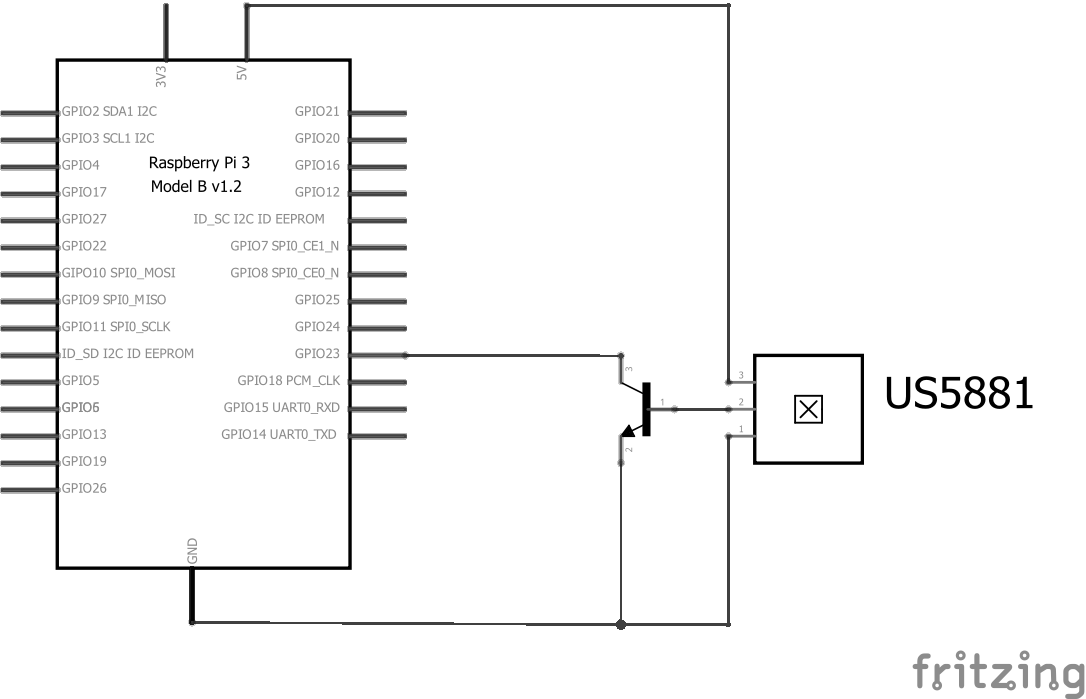
\includegraphics[scale=0.3]{images/circspeeddet.png}
	\caption{Hall Effect Speed Detector Circuit Diagram}
	\label{circhall}
\end{figure} \newline  \noindent
This circuit does not measure the instantaneous rotational speed of the motor. Instead it measures the average speed. By using more magnets, and a smaller time-frame, the speed measured becomes closer to an instantaneous speed. The advantage of using this circuit is that it is simple to set up and use, other speed detection circuits require the use of lasers and photodiodes/phototransistors, or dc dynamos and analogue to digital converters. However, the main downside lies in having to attach magnets at regular intervals to the rotating cylinder, which will have to be done accurately. Another downside is the range of the hall effect sensor. The sensor must be within 10mm of the magnet for it to be able recognise it. \newline \newline \noindent
\large Light Sensor \normalsize \br
The rotational speed of the motor was measured using a light-gate type set up. An IR-LED and IR-phototransistor were set up near the inner cylinder. A metal trip was attached to the cylinder such that it broke the light beam between the LED and the phototransistor. The transistor was set up as a switch such that when light was allowed to fall onto the transistor, a complete circuit was made between GPIO23 (pulled high by the build in resistor) and ground on the Raspberry pi, thus a low value is read. When the beam is broken, this circuit breaks too, causing the value of GPIO23 to go high. On the software side, this value change can be detected and the timing of which can be used to calculate the speed. \newline

\end{document}